% https://www.dfg.de/formulare/54_01/54_01_de.pdf
\documentclass[11pt,a4paper]{article}

\usepackage{SmallCaption}
%\usepackage{ngerman}
%\usepackage[german]{babel}
%\usepackage[dvips,final]{epsfig}
%\usepackage{german}
\usepackage{a4}
\usepackage{graphicx}
%\usepackage{natbib}

%\usepackage{biblatex}
%\defbibheading{empty}[]{}

\usepackage[utf8]{inputenc}
%\usepackage[latin1]{inputenc}
\usepackage{amsmath}
\usepackage{amsthm}
\usepackage{amssymb}
\usepackage{array}
\usepackage{enumitem}
\usepackage{footmisc}

\usepackage{graphics}
\usepackage{xcolor}
%\usepackage{a4wide}
%\usepackage{pstricks}
%\usepackage{pst-node}
%\usepackage{multido}
\usepackage{url}

%\usepackage{fancybox}
%\usepackage{multirow}
%\usepackage{psboxit}
%\usepackage{graphicx}

%\usepackage{float}
%\usepackage{bm}
%\usepackage{ifthen}
%\usepackage{url}
%\usepackage{hyperref}
%\usepackage{epsfig}
%\usepackage{fancyhdr}

\frenchspacing
%% Hoehe um 20mm vergroessern
%\addtolength{\topmargin}{-10mm} \addtolength{\textheight}{15mm}
%% Breite um 12mm vergroessern
%\addtolength{\oddsidemargin}{-6mm} \addtolength{\evensidemargin}{-6mm}
%\addtolength{\textwidth}{12mm}

%% Hoehe um 20mm vergroessern
%\addtolength{\topmargin}{-10mm} \addtolength{\textheight}{15mm}
%% Breite um 24mm vergroessern
%\addtolength{\oddsidemargin}{-10mm} \addtolength{\evensidemargin}{-10mm}
%\addtolength{\textwidth}{20mm}


% Hoehe um 20mm vergroessern
\addtolength{\topmargin}{-20mm} \addtolength{\textheight}{30mm}
% Breite um 30mm vergroessern
\addtolength{\oddsidemargin}{-15mm} \addtolength{\evensidemargin}{-15mm}
\addtolength{\textwidth}{35mm}


\setlength{\parindent}{0cm}
\pagestyle{empty}
%\pagestyle{plain}
\setcounter{secnumdepth}{5}

\parindent 0mm
\parskip \medskipamount
\def\F{{\mathbb F}}
\def\N{{\mathbb N}}
\def\Z{{\mathbb Z}}
\def\Q{{\mathbb Q}}
\def\R{{\mathbb R}}
\def\C{{\mathbb C}}
\def\K{{\mathbb K}}
\def\G{\mathbb{G}}
\def\H{\mathbb{H}}
\def\PN{\mathrm{ISAD}}

\newcommand{\iec}{i.e.,\ }
\newcommand{\ie}{i.e.\ }
\newcommand{\egc}{e.g.,\ }
\newcommand{\eg}{e.g.\ }

\newcommand{\MATLAB}[0]{MATLAB}
\newcommand{\supress}[1]{}

\newcommand{\mm}[1]{{\bf #1}}
\newcommand{\mc}[1]{{\bf #1}}

\newenvironment{itemizePacked}{
\begin{itemize}
  \setlength{\itemsep}{1pt}
  \setlength{\parskip}{0pt}
  \setlength{\parsep}{0pt}
  \renewcommand{\labelitemi}{$\bullet$}
}{\end{itemize}}

\newenvironment{itemizePacked2}{
\begin{itemize}
  \setlength{\itemsep}{1pt}
  \setlength{\parskip}{0pt}
  \setlength{\parsep}{0pt}
  \renewcommand{\labelitemi}{$-$}
}{\end{itemize}}

%\newrgbcolor{christianColor}{0 0.7 0}
%\newrgbcolor{meinardColor}{1 0 1}
%\newrgbcolor{haraldColor}{0 0.6 1}
%\newrgbcolor{nanzhuColor}{0.7 0.7 0}
%\newcommand{\sebastian}[1]{ {\color{sebastianColor} #1} }
%\newcommand{\meinard}[1]{ {\color{meinardColor} #1} }

\newcommand{\meinard}[1]{{\color{red} #1}}
\newcommand{\jakob}[1]{{\color{magenta} #1}}
\newcommand{\yigit}[1]{{\color{orange} #1}}
\newcommand{\krause}[1]{{\color{brown} #1}}
\newcommand{\taenzer}[1]{{\color{green} #1}}
\newcommand{\christof}[1]{{\color{blue} #1}}


%%%%%%%%%%%%%%%%%%%%%%%%%%%%%%%%%%%%%%%%%%%%%%%%%%%%%%%%%%%%%%%%%%%%%%%%%%%%
\theoremstyle{plain} \newtheorem{define}{Definition}[section]
\renewcommand{\familydefault}{\sfdefault}

\begin{document}
\sloppy


%%%%%%%
%\subsection*{Macros for Authors/Instructions}
%\begin{itemizePacked}
%\item \meinard{Macro for Meinard.}
%\item \jakob{Macro for Jakob.}
%\item \yigit{Macro for Yigit.}
%\item \krause{Macro for Michael Krause.}
%\item \taenzer{Macro for Michael Taenzer.}
%\item \christof{Macro for Christof.}
%\item General Information: 1 page
%\item Section 1: 8 pages
%\item Section 2: 5 pages
%\item Section 3: 2 pages
%\item Section 4 - 7: 4 pages
%\item Zoom Meeting (Meinard):\\
%\url{https://fau.zoom.us/j/9681879392?pwd=M0drcTF6MU4zNUQ4eUxJT3AvdUl3dz09}\\
%\url{Meeting ID: 968 187 9392}\\
%\url{Password: 017498}
%\item \url{https://www.overleaf.com/7585719473jkmzsvhwzsdk}
%\end{itemizePacked}
%
%\subsubsection*{Informierte Klangquellenerkennung in Musik- und Audiosignalen}
%
%Im Bereich des ``Music Information Retrieval'' (MIR) ist die Entwicklung von computergestützten Methoden zur Analyse, Segmentierung und Klassifizierung von Musiksignalen von grundlegender Bedeutung. In der ersten Phase dieses Projekts (Erstantrag) untersuchten wir grundlegende Techniken zur Erkennung charakteristischer Klangereignisse, die in einer gegebenen Musikaufnahme vorhanden sind. Dabei lag unser Fokus auf Ansätzen, die musikalisches Wissen in Form von Notentextinformationen, Klangbeispielen oder musikalisch repräsentativen Musikpassagen nutzen. Zentrale Aufgabenstellungen bestanden im Auffinden von Audioabschnitten mit einer bestimmten Klangfarbe oder Instrumentierung, die Erkennung monophoner Themen in polyphonen Musikaufnahmen und die Klassifizierung von Musikstilen oder Spielweisen anhand melodischer Konturmerkmale. Die entwickelten Erkennungsverfahren wurden im Rahmen komplexer Musikszenarien (u.a. klassische Musik, Jazzmusik und Opernaufnahmen) experimentell getestet und ausgewertet. 
%%
%In der zweiten Projektphase (Verlängerungsantrag) erweitern wir unsere Ziele erheblich. Erstens betrachten wir neben dem Musikszenario die Erkennung von Umwelt- und Umgebungsgeräusche als zweite komplexe Audiodomäne. Zweitens wollen wir, als unsere zentrale Methodik, Aspekte von modellbasierten und datengetriebenen Verfahren kombinieren, um aufgabenspezifische Darstellungsformen von Klangereignissen zu lernen. Darüber hinaus werden wir integrative und hierarchische Strategien verfolgen, um Schallereignisse auf verschiedenen Zeitskalen und hinsichtlich hierarchisch angeordneter Kategorien zu erfassen und zu analysieren. Unser übergeordnetes Ziel der zweiten Projektphase ist es, erklärbare und nachvollziehbare Deep-Learning-Modelle zu entwickeln, die ein besseres Verständnis der strukturellen und akustischen Eigenschaften von Klangquellen ermöglichen.
%
%
%\pagebreak[4]
%%%%%%%


\begin{center}
%\bf Fortsetzungsantrag, Deutsche Forschungsgemeinschaft (DFG)
\bf Renewal Proposal, Deutsche Forschungsgemeinschaft (DFG)
\end{center}

%%%%%%%%%%%%%%%%%%%%%%%%%%%%%%%%%%%%%%%%%%%%%%%%%%%%%%%%%%%%%%%%%%%%%%%%%%%%

%\newpage
%\tableofcontents

%%%%%%%%%%%%%%%%%%%%%%%%%%%%%%%%%%%%%%%%%%%%%%%%%%%%%%%%%%%%%%%%%%%%%%%%%%%%

%\newpage


%%%%%%%%%%%%%%%%%%%%%%%%%%%%%%%%%%%%%%%%%%%%%%%%%%%%%%%%%%%%%%%%%%%%%%%%%%%%

%\newpage
%\tableofcontents

%%%%%%%%%%%%%%%%%%%%%%%%%%%%%%%%%%%%%%%%%%%%%%%%%%%%%%%%%%%%%%%%%%%%%%%%%%%%

%\setcounter{page}{1}

%%%%%%%%%%%%%%%%%%%%%%%%%%%%%%%%%%%%%%%%%%%%%%%%%%%%%%%%%%%%%%%%%%%%%
%%%%%%%%%%%%%%%%%%%%%%%%%%%%%%%%%%%%%%%%%%%%%%%%%%%%%%%%%%%%%%%%%%%%%
% Abschnitt 1. Allgemeine Angaben             1111111111111
%%%%%%%%%%%%%%%%%%%%%%%%%%%%%%%%%%%%%%%%%%%%%%%%%%%%%%%%%%%%%%%%%%%%%
%%%%%%%%%%%%%%%%%%%%%%%%%%%%%%%%%%%%%%%%%%%%%%%%%%%%%%%%%%%%%%%%%%%%%

\vspace{-0.0cm}


%%%%%%%%%%%%%%%%%%%%%%%%%%%%%%%%%%%%%%%%%%%%%%%%%%%%%%%%%%%%%%%%%%%%%
\section*{General Information}
%%%%%%%%%%%%%%%%%%%%%%%%%%%%%%%%%%%%%%%%%%%%%%%%%%%%%%%%%%%%%%%%%%%%%

\vspace{-0.5cm}

\begin{tabbing}
\hspace{3cm}\= \\ \kill
Name:\>{\bf Prof. Dr. rer. nat. Meinard M\"uller} \\
Position:\> Professor (W3, permanent) f\"ur Semantische Audiosignalverarbeitung\\
%Date of Birth:\>19.08.1969\\
Nationality:\>German \\
Institution:\>Friedrich-Alexander-Universit\"at Erlangen-N\"urnberg\\
Address (work):\>Am Wolfsmantel 33, 91058 Erlangen\\
Phone:\> +49 9131 85-20504\\
%Fax:\> +49 9131 85-20524\\
E-mail:\>{\tt meinard.mueller@audiolabs-erlangen.de} \\
%Address (private):\>An der Wied 19a, 91058 Erlangen\\
%Phone:\> +49 9131 4008768\\
%Reference number of a previous DFG grant proposal: MU~2686/3-1\\
\end{tabbing}

\vspace{-1.5cm}

\begin{tabbing}
\hspace{3cm}\= \\ \kill
Name:\>{\bf Dr.-Ing. Jakob Abe{\ss}er} \\
Position:\> Senior Scientist\\
%Date of Birth:\>03.05.1983\\
Nationality:\>German \\
Institution:\>Fraunhofer Institut f\"ur Digitale Medientechnologie (IDMT)\\
Address (work):\>Ehrenbergstra{\ss}e 31, 98693 Ilmenau\\
Phone:\> +49 3677 467288 \\
%Fax:\> +49 3677 467467 \\
E-mail:\>{\tt jakob.abesser@idmt.fraunhofer.de} \\
%Address (private):\>Annemarie-Becker-Straße 16, 99092 Erfurt\\
%Phone:\>+49 176 61104420\\
%Reference number of a previous DFG grant proposal: AB 675/2-1\\
\end{tabbing}

\vspace{-0.5cm}

%{\bf Topic:} Source \underline{Se}paration and \underline{Re}storation of Drum Sound \underline{Co}mponents in Music Recordings
{\bf Topic (initial proposal, MU 2686/11-1, AB 675/2-1):} \underline{I}nformed \underline{S}ound \underline{A}ctivity \underline{D}etection in Music Recordings 

{\bf Topic (renewal proposal):} \underline{I}nformed \underline{S}ound \underline{A}ctivity \underline{D}etection in Music and Audio Signals

{\bf Project Name:} $\PN$

%
% Bem.: "Kennwort." ist lt. DFG-Leitfaden nicht mehr vorgesehen
%

{\bf Subject Area:} Computer Science, Artificial Intelligence, Image and Language Processing

{\bf Keywords:} Music Processing, Audio Processing, Music Information Retrieval

{\bf Duration (in months):} 36 (Renewal Proposals)


% Informed Sound Activity Detection in Music and Environmental Signals 
%06 Generalization Towards other Audio Domains
%07 Representation Learning ...
%08 Hierarchical Approaches ...
%09 Towards Sound Event Understanding 


{\bf Summary:}
%
%nicht mehr als 15 Zeilen (max. 1600 Zeichen)
%
% Summary of initial proposal
%In music information retrieval, the development of computational methods for analyzing, segmenting, and classifying music signals is of fundamental importance. One prominent task is known as singing voice detection. The objective is to automatically locate all sections of a given music recording where a main singer is active. Although this task seems to be simple for human listeners, the detection of the singing voice by computational methods remains difficult due to complex superpositions of sound sources that typically occur in music where the singing voice interacts with accompanying instruments. Extending this scenario, the goal of automatic instrument recognition is to identify all performing instruments in a given music recording and to derive a segmentation into sections with homogeneous instrumentation. Other related problems deal with finding all monophonic sections, identifying all solo parts or sections with a predominant melody, or locating sections with a specific timbre. In this project, motivated by these segmentation problems, we want to adopt a comprehensive perspective. Our goal is to explore fundamental techniques and computational tools for detecting sound sources or characteristic sound events that are present in a given music recording. To cope with a wide range of musical properties and complex superpositions of different sound sources, we want to focus on informed approaches that exploit various types of additional knowledge. Such knowledge may be given in the form of musical parameters (\egc number of instruments, score information), sound examples (\egc instrument samples, representative sections), or user input (\egc annotations, interactive feedback). By combining audio segmentation, detection, and classification techniques, one main objective is to develop novel approaches that can efficiently adapt to requirements within specific application scenarios. To test and evaluate our activity detection algorithms, we consider various challenging music scenarios including Western classical music, jazz music, and opera recordings.
%
%New Objectives:
%Generalization Towards other Audio Domains.
%Representation Learning
%Hierarchical Approaches
%Towards Sound Event Understanding
%
In music information retrieval (MIR), the development of computational methods for analyzing, segmenting, and classifying music signals is of fundamental importance. In this project's first phase (initial proposal), we explored fundamental techniques for detecting characteristic sound events present in a given music recording. Here, our focus was on informed approaches that exploit musical knowledge in the form of score information, instrument samples, or musically salient sections. We considered concrete tasks such as locating audio sections with a specific timbre or instrument, identifying monophonic themes in complex polyphonic music recordings, and classifying music genres or playing styles based on melodic contours. We tested our approaches within complex music scenarios, including instrumental Western classical music, jazz, and opera recordings.
%
In the second phase of the project (renewal proposal), our goals will be significantly extended. First, we want to go beyond the music scenario by considering environmental sounds as a second challenging audio domain. As a central methodology, we plan to explore and combine the benefits of model-based and data-driven techniques to learn task-specific sound event representations. Furthermore, we will investigate hierarchical approaches to simultaneously incorporate, exploit, learn, and capture sound events that manifest on different temporal scales and belong to hierarchically ordered categories. An overarching goal of the project's second phase is to develop explainable deep learning models that provide a better understanding of the structural and acoustic properties of sound events.
%
%Finally, by considering two distinct audio domains, the general goals of the project's second phase are to gain a deeper understanding of the structural properties of sound events and to obtain explainable deep learning models that are less vulnerable to data biases and confounding factors. 
\pagebreak[4]\clearpage

\sloppy \pagestyle{plain} \setcounter{page}{1}

%%%%%%%%%%%%%%%%%%%%%%%%%%%%%%%%%%%%%%%%%%%%%%%%%%%%%%%%%%%%%%%%%%%%%
\section*{Project Description}
%%%%%%%%%%%%%%%%%%%%%%%%%%%%%%%%%%%%%%%%%%%%%%%%%%%%%%%%%%%%%%%%%%%%%

%%%%%%%%%%%%%%%%%%%%%%%%%%%%%%%%%%%%%%%%%%%%%%%%%%%%%%%%%%%%%%%%%%%%%
\section*{1 Starting point}
%%%%%%%%%%%%%%%%%%%%%%%%%%%%%%%%%%%%%%%%%%%%%%%%%%%%%%%%%%%%%%%%%%%%%
%\info{For renewal proposals, please report on your previous work. This report should also be understandable without referring to additional literature.}

In the following, we report on our main project-related achievements over the last years. This description also constitutes the state of the art and preliminary work for the renewal proposal. More specifically, we first summarize the central results of the project's first phase (period from November 2017 to July 2021). Then, we give an overview of the project employees and discuss their respective qualifications and contributions. Next, we provide an overview of collaborations, activities, demonstrators, and source code made available in the $\PN$~project. Subsequently, we discuss deviations from the initial work plan and indicate follow-up examinations, which also motivate the objectives of the renewal proposal.
%
We refer to the initial proposal for a detailed description of the general state of the art and prior work. We extend this description by discussing relevant work in 
%acoustic scene classification and 
environmental sound analysis while summarizing important recent developments in deep learning that form the technical basis for our investigations intended in the second phase of the $\PN$~project. Finally, in Section 1.2, we list the most important publications of the project's first phase.
%
At this point, we want to emphasize that (besides the research-related aspects) we see education and training of the next generation of scientists as another central element of the $\PN$~project.

%%%%%%%%%%%%%%%%%%%%%%%%%%%%%%%%%%%%%%%%%%%%%%%%%%%%%%%%%%%%%%%%%%%%%
\section*{1.1 State of the art and preliminary work}
%%%%%%%%%%%%%%%%%%%%%%%%%%%%%%%%%%%%%%%%%%%%%%%%%%%%%%%%%%%%%%%%%%%%%

%%%%%%%%%%%%%%%%%%%%%%%%%%%%%%%%%%%%%%%%%%%%%%%%%%%%%%%%%%%%%%%%%%%%%
\subsubsection*{Initial objectives and results achieved (initial application)}
%%%%%%%%%%%%%%%%%%%%%%%%%%%%%%%%%%%%%%%%%%%%%%%%%%%%%%%%%%%%%%%%%%%%%

The general goal of the initial $\PN$~project was to develop techniques and tools for analyzing, segmenting, and classifying music signals according to various sound characteristics. In particular, we considered detecting specific sound events related to singing voices, certain instruments, or specific musical themes. 
%
In the initial proposal, we considered five objectives. In the first three objectives [O1], [O2], and [O3], we considered specific segmentation and classification subtasks related to sound event activity detection. Then, we addressed in objective [O4] the general aspect of knowledge integration and covered in objective [O5] various application scenarios. We now summarize, along with these objectives, the main results that we achieved in the reporting period from November 2017 to July 2021. Many of the key findings of the $\PN$~project are based on the publications listed in Section 1.2.  

\begin{enumerate}
%%%%%%%%%%%%%%%%%%%%%%%%%%%%%%%%%%%%%%%%%%%%%%%%%%
\item [\textbf{[O1]}] \textbf{Detection of Characteristic Sound Events.}
%
%The presence of a particular instrument or a singing voice is often correlated to specific sound events or characteristic spectro-temporal patterns. In this objective, we studied computational approaches for detecting sound events that are contained in complex sound mixtures. 
%
%\textbf{Achievements:}
%
%\begin{itemizePacked}
%\item \cite{ZalkowM20_WeaklyAlignedTrain_ISMIR}
%\item Structure boundaries in Jazz recordings
%\end{itemizePacked}
%
In the $\PN$-project, we explored a range of different sound event detection problems using traditional model-based as well as data-driven machine learning approaches. In~\cite{Reck19_StructureBoundary_MasterThesis}, we investigated and compared such approaches for detecting musical boundaries in jazz audio recordings. As we further discuss in the subsequent paragraphs (see [O2] and [O3]), we considered detection scenarios for singing voice in opera recordings~\cite{KrauseMW21_OperaSingingActivity_Electronics,MimilakisWAAM19_SingingVDetWagner_MML} and for instrument families in instrumental music~\cite{TaenzerAMWLM19_InstrumentReco_ISMIR}. In~\cite{AbesserMueller19_ContourClassification_ICASSP}, we looked at contours of frequency trajectories as characteristics of sound events and used derived audio features for various classification applications (see also [O3]).
%
Within the broader context of sound event detection, we considered in~\cite{ZalkowM20_WeaklyAlignedTrain_ISMIR} a particularly challenging pattern detection task. Given a specific musical theme that expresses a characteristic musical idea (in our case, we used short monophonic symbolically encoded musical themes), the objective is to retrieve all music recordings from an audio database where this theme is played (see also [O5]). Note that musical themes are typically accompanied and superimposed with other musical sources, thus being embedded into complex sound mixtures. This makes their detection a challenging problem.
%
As our main contribution for solving this cross-modal detection task, we applied deep learning techniques to learn suitable mid-level representations. In particular, we employed the Connectionist Temporal Classification (CTC) loss to learn such representations from weakly aligned score--audio pairs (thus avoiding the need for strongly aligned training data, which are hard to obtain).  
%
%We conducted extensive experiments that show the effectiveness of the CTC-based model for this theme detection task 
%
A vastly extended version of~\cite{ZalkowM20_WeaklyAlignedTrain_ISMIR} is currently in the revision process~\cite{ZalkowM21_CTC-Chroma_TASLP} and is also a main part of the first author's Ph.D. thesis~\cite{Zalkow21_LearningAudioRep_PhD}.

%%%%%%%%%%%%%%%%%%%%%%%%%%%%%%%%%%%%%%%%%%%%%%%%%%
\item [\textbf{[O2]}] \textbf{Segmentation of Complex Sound Mixtures.}
%
%Given a music recording, segmentation may be described as the process of partitioning the audio stream into sections that are of musical/acoustical relevance and that are somehow easier to understand than the original recording. In this objective, our goal was to segment a given music recording into (homogeneous) sections that indicate the presence or absence of certain instruments or other sound events.
%
%\textbf{Achievements:}
%\begin{itemizePacked}
%\item \cite{MimilakisWAAM19_SingingVDetWagner_MML} 
%\item \cite{KrauseMW21_OperaSingingActivity_Electronics}
%\item \cite{ZalkowBM19_SalienceRetrieval_ICASSP}
%\item \cite{AbesserBM18_BassSaliency_ISMIR} - \jakob{studied label propagation to transfer bass pitch annotations to unlabeled datasets, studied different transfer learning approaches to combine bass transcription for isolated bass notes and bass lines within ensemble recordings.}
%\item \cite{AbesserM21_JazzBassTranscription_Electronics} - \jakob{achieved a new state-of-the-art for jazz bass transcription by transferring a recently proposed u-net convolution neural network architecture for melody transcription to learn a mapping from constant-Q spectra to bass pitch activities. An advantage of this model is that it implicitly learns to model the bass instrument activity in its bottleneck layer. }
%\end{itemizePacked}
%
As already indicated in [O1], we investigated in the $\PN$-project several problems related to music segmentation with the objective to partition a  music recording into (homogeneous) sections that indicate the presence or absence of specific instruments or other sound events. 
%
In~\cite{KrauseMW21_OperaSingingActivity_Electronics,MimilakisWAAM19_SingingVDetWagner_MML}, we considered the case of detecting sections with singing voice. Applied to complex opera recordings, we explored traditional machine learning techniques based on random forests and hand-engineered features as well as end-to-end deep learning approaches. Using novel data splitting strategies that can be applied in particular for Western classical music (exploiting the existence of multiple performances for the same piece of music, see also [O4]), we obtained a deeper understanding of the benefits and limitations of the different approaches. 
%
In~\cite{AbesserBM18_BassSaliency_ISMIR,AbesserM21_JazzBassTranscription_Electronics}, we used pitch-saliency measures to identify segments where the bass instrument is active. Looking at jazz ensemble recordings, we were particularly interested in identifying and transcribing the bass line. As the main contribution of~\cite{AbesserBM18_BassSaliency_ISMIR}, we conducted experiments using transfer learning, where we first trained models using isolated note recordings and then refined these models for the task of detecting bass activity sections in complex music mixtures.
%
In~\cite{AbesserM21_JazzBassTranscription_Electronics}, we achieved state-of-the-art results for jazz bass transcription by adapting recently proposed U-Net neural network architectures (initially used for melody transcription). An important insight is that we could use the same model to improve on the bass activity detection task by looking at the U-Net's bottleneck layer.

%%%%%%%%%%%%%%%%%%%%%%%%%%%%%%%%%%%%%%%%%%%%%%%%%%
\item [\textbf{[O3]}] \textbf{Sound Event Classification and Automatic Instrument Recognition.}
%
%Besides \emph{detection} (see [O1]) and \emph{segmentation} (see [O2]), the \emph{classification} of the detected sound events and segments according to musically meaningful categories is another fundamental issue. In this objective, we addressed different classification problems where these categories comprise instruments and singing voices as well as categories on a higher hierarchical level such as instrument families.
%
%\textbf{Achievements:}
%\begin{itemizePacked}
%\item \cite{TaenzerAMWLM19_InstrumentReco_ISMIR} - \jakob{instrument family recognition in classicial music, particular focus was on studying the influence of data normalization, pre-processing and data ugmentation of the performance of a CNN model. Furthermore, cross-dataset experiments revealed the necessity of further domain adaptation.}
%\item \cite{TaenzerMA21_LocalPolyphonyEstimation_Electronics} - \jakob{studied CNN-based estimation of local polyphony in piano recordings and its application as a post-processing filter to select note candidates for multi-pitch estimation. In-depth comparison of different feature representation and network architectures.}
%\item \cite{AbesserMueller19_ContourClassification_ICASSP} - \jakob{comparative study between hand-crafted and CNN-based (learnt) audio features to characterize f0 contour shapes for four different classification tasks.}
%\item \cite{WeissBAM18_JazzComplexity_ISMIR}: Harmonic complexity
%\item \jakob{\cite{Gomez:2018:IREC:ISMIR}}: 
%\item \jakob{\cite{AbesserCTPM21_InstrumentJazz_EUSIPCO} - predominant instrument recordings using a CNN model, we studied harmonic/percussive as well as solo/accompaniment source separation as pre-processing step to improve the instrument recognition performance, for solo instrument recogntiion in jazz ensemble recordings, we studied transfer learning.}  
%\item \jakob{predominant instrument recognition in jazz recordings, comparison of three SOTA CNN models and different dataset-split strategies}
%% TBD (will be submitted on 15.6.) \item \jakob{\cite{MimilakisTA21_InstrumentReco_CMMR}} (submitted)
%\item , while in \cite{TaenzerAMWLM19_InstrumentReco_ISMIR} our goal was to identify sections with certain instrumentation. These approaches will be further discussed in the context of subsequent objectives. 
%\end{itemizePacked}
%
Besides \emph{detection} (see [O1]) and \emph{segmentation} (see [O2]), the \emph{classification} of the detected sound events and segments according to musically meaningful categories is another fundamental issue addressed in the $\PN$-project. In the following, we summarize our main contributions in this context.
%
First, in~\cite{TaenzerAMWLM19_InstrumentReco_ISMIR}, we considered the task of instrument family recognition, applying it mainly to recordings of Western classical music. While using standard CNN-based learning techniques, we explored the potential of data normalization, preprocessing, and data augmentation techniques within this challenging classification scenario. In particular, our cross-dataset experiments showed the importance of data augmentation and normalization techniques to achieve good generalization.
%
Second, in~\cite{TaenzerMA21_LocalPolyphonyEstimation_Electronics}, we studied the task of estimating the degree of local polyphony in piano recordings and its application for polyphony-informed multi-pitch estimation. In this context, we conducted an in-depth comparison of different feature representations and network architectures.
%
Third, we applied in~\cite{AbesserCTPM21_InstrumentJazz_EUSIPCO} audio decomposition techniques (in particular, harmonic--percussive and solo--accompaniment separation) as preprocessing step to improve solo-instrument recognition in jazz music.  
%
In a follow-up study~\cite{AbesserCTPM21_InstrumentJazz_EUSIPCO}, we systematically explored different CNN-based architectures for an extended taxonomy of predominant instruments in jazz music.
%
Finally, we compared in~\cite{AbesserMueller19_ContourClassification_ICASSP} hand-crafted and learned feature representations (using CNN models) for characterizing fundamental frequency shapes (also called contours), which were applied to different tasks such as genre, instrument, and playing style classification. 

%%%%%%%%%%%%%%%%%%%%%%%%%%%%%%%%%%%%%%%%%%%%%%%%%%
\item [\textbf{[O4]}] \textbf{Integration of Additional Knowledge.}
%
%In this objective, we considered different strategies for incorporating prior knowledge to simplify the segmentation, detection, and classification tasks as specified in the previous objectives.
%
%\textbf{Achievements:}
%\begin{itemizePacked}
%\item \cite{AbesserMueller19_ContourClassification_ICASSP}
%\item \cite{TaenzerMA21_LocalPolyphonyEstimation_Electronics} - \jakob{}
%\item ...
%\end{itemizePacked}
%
Together with the music recording to be analyzed, one often has additional knowledge on the type of music being played or the sounds to be expected. In the $\PN$-project, we integrated such knowledge in various ways.
%
In~\cite{ZalkowM20_WeaklyAlignedTrain_ISMIR}, the sound events (musical themes) were specified in a symbolic format. This symbolic information was used to guide our learning procedure to derive mid-level representations. In this process, to avoid the need for strong (\iec frame-wise) alignments, we applied techniques that only require weak alignments (see also [O1]). 
%
In~\cite{TaenzerAMWLM19_InstrumentReco_ISMIR}, we considered an informed classification scenario, where the classes were assembled according to instrument families (\egc strings, woodwind, brass, percussion). In the new objective [O8] (see Section 2.2), we plan to systematically carry out the idea of exploiting hierarchically ordered categories.
%
%In our studies~\cite{KrauseMW21_OperaSingingActivity_Electronics,MimilakisWAAM19_SingingVDetWagner_MML}, we gained more profound insights into scalability and generalizability properties of machine learning approaches by considering novel data splits that exploit the availability of multiple performances of the same musical piece (in our case operas).
%
In many of our data-driven procedures, we applied acoustically and musically informed data augmentation techniques such as simulating room impulse responses in~\cite{TaenzerAMWLM19_InstrumentReco_ISMIR} or applying pitch shifting and time stretching in~\cite{AbesserBM18_BassSaliency_ISMIR}.
%
In~\cite{ZalkowBM19_SalienceRetrieval_ICASSP}, we compared melody-enhanced salience representations in the context of a cross-modal retrieval application. 
%
As a powerful yet little-studied research direction, we adopted in~\cite{KrauseMW21_OperaSingingActivity_Electronics,MimilakisWAAM19_SingingVDetWagner_MML} a cross-version learning approach that exploits the availability of multiple versions (in our case performances) of the same musical work (in our case operas).% 
%This strategy may be interpreted as a musically informed data augmentation scenario. 
%
Considering novel data splits across versions yields deep insights into the stability and generalizability of deep learning models---a research direction we want to investigate further in the second phase of the $\PN$-project.



%%%%%%%%%%%%%%%%%%%%%%%%%%%%%%%%%%%%%%%%%%%%%%%%%%
\item [\textbf{[O5]}] \textbf{Applications in Complex Music Scenarios.}
%
%In this objective, we tested and evaluated our activity detection algorithms by considering various challenging music scenarios including Western classical music, jazz music, and opera recordings.
%
%\textbf{Achievements:}
%\begin{itemizePacked}
%\item \cite{KrauseMW21_OperaSingingActivity_Electronics}: Wagner dataset
%\item \cite{ZalkowBAM20_MTD_TISMIR}: MTD dataset
%\item WJD: Jazz dataset with structure annotations; publication in preparation
%\item \cite{WeissBAM18_JazzComplexity_ISMIR}
%\end{itemizePacked}
%
As one challenging music scenario, we created within the $\PN$-project a multimodal dataset referred to as Musical Theme Dataset (MTD), which we used to evaluate our theme-based sound event detection approach~\cite{ZalkowM20_WeaklyAlignedTrain_ISMIR} (see also [O1]). The MTD consists of 2067 musical themes that are prominent in Western classical music. For each of the themes, the MTD provides symbolic music encodings, audio snippets of music recordings, alignments between the symbolic and audio representations, as well as detailed metadata on the composer, work, recording, and musical characteristics of the themes. In addition, we also developed several parsers and web-based interfaces for accessing and exploring the various data modalities and their relations through visualizations and sonifications. To foster open source and reproducible research, we made the MTD and the software publicly available while indicated its potential for music information retrieval (MIR) research. The documentation and possible applications can be found in the journal publication~\cite{ZalkowBAM20_MTD_TISMIR}, which we consider a significant contribution of the $\PN$-project.
%
For singing voice and instrument recognition, we used in our experiments MIR datasets that mainly comprise popular music as well as a newly created dataset with opera recordings~\cite{KrauseMW21_OperaSingingActivity_Electronics,MimilakisWAAM19_SingingVDetWagner_MML} and Western instrumental music~\cite{TaenzerAMWLM19_InstrumentReco_ISMIR}.   
%
Beyond Western classical and popular music, we considered in~\cite{AbesserBM18_BassSaliency_ISMIR,
AbesserMueller19_ContourClassification_ICASSP,
Reck19_StructureBoundary_MasterThesis,
WeissBAM18_JazzComplexity_ISMIR}  jazz music as another challenging genre. We made the annotations used for our bass transcription experiments publicly available. Furthermore, extending~\cite{Reck19_StructureBoundary_MasterThesis}, we are currently preparing a dataset publication that makes other boundary, structure, and instrumentation annotations (along with open-source implementations of baseline algorithms) available.
\end{enumerate}

%\begin{figure}[t]
%\begin{center}
%\includegraphics[width=14cm]{figures/Figure.png}
%\end{center}
%\vspace{-0.3cm}
%\caption{Overview. \textbf{(a)}
%\textbf{(b)}
%}
%\label{figures:text}
%\end{figure}

%%%%%%%%%%%%%%%%%%%%%%%%%%%%%%%%%%%%%%%%%%%%%%%%%%%%%%%%%%%%%%%%%%%%%
\subsubsection*{Project employees, qualification of young scientists, contributions}
\label{sec:employees}
%%%%%%%%%%%%%%%%%%%%%%%%%%%%%%%%%%%%%%%%%%%%%%%%%%%%%%%%%%%%%%%%%%%%%

The initial $\PN$~project was approved for $36$ months, providing funds for two full positions---one for Erlangen (FAU) and one for Ilmenau (IDMT). The following list gives an overview of the project's employees as well as the funding periods and volumes (in employee months). Note that most project members were funded only partly by the $\PN$-project and partly by other funds (including interruptions due to parental leave, internships, and more extended research stays).

{\small
\begin{itemizePacked}
\item Frank Zalkow (Erlangen, FAU), 01.11.2017 -- 31.07.2021 (ca. 50\,\%,  23 months in total)
\item Michael Krause (Erlangen, FAU), 01.03.2020 -- 31.12.2020 (50\,\%, 5 months in total)
\item Christof Wei{\ss} (Erlangen, FAU), 01.09.2018 -- 30.06.2019 (50\,\%, 5 months in total)
\item Stefan Balke (Erlangen, FAU), 01.11.2017 -- 30.06.2018 (ca. 50\,\%, 3 months in total)
\item Michael Taenzer (Ilmenau, IDMT), 01.05.2018 -- 31.04.2021 (ca. 50\,\%, 20 months in total)
\item Stylianos Mimilakis (Ilmenau, IDMT), 01.08.2018 -- 31.04.2021 (ca. 50\,\%, 16 months in total)
\end{itemizePacked}
}


% Michael Taenzer (tzr)
% 2021: Jan-April 4
% 2020: Jan-Nov 11
% 2019: Jan-Dez 12
% 2018: Mai-Dez 8

% und 

% Stylianos Mimilakis (mis)
% 2021: Jan-April 4
% 2020: Jan-Nov 11
% 2019: Jan – Juni und Okt-Dez 9
% 2018: Aug-Dez 5



%\vspace{-4mm}
%
%\begin{tabbing}
% \hspace{6.5cm} \= \hspace{4.5cm} \=\kill\\
% Frank Zalkow (Erlangen, FAU)\>  01.11.2017 -- 31.07.2021\> (ca. 50\,\%,  23 months)\\%[1mm]
% Michael Krause (Erlangen, FAU)\>  01.03.2020 -- 31.12.2020 \> (50\,\%, 5 months)\\%[1mm] 
% Christof Wei{\ss} (Erlangen, FAU)\>  01.09.2018 -- 30.06.2019 \> (50\,\%, 5 months)\\%[1mm]
% Stefan Balke (Erlangen, FAU)\>  01.11.2017 -- 30.06.2018 \> (ca. 50\,\%, 3 months)%[1mm]
%\end{tabbing}
%\vspace{-4mm}
%
%Frank Zalkow, E 13 (50% + 50%), 01.11.2017 - 31.12.2017, DFG AnChor + DFG ISAD
%Frank Zalkow, E 13 (full), 01.01.2018 - 31.12.2018, (50% + 50%), DFG AnChor + DFG ISAD
%Frank Zalkow, E 13 (full), 01.01.2019 - 28.02.2019, 01.06.- 31.10.2019, (50% + 50%), DFG AnChor + DFG ISAD
%Frank Zalkow, E 13 (full), 01.01.2020 - 31.10.2020, (50% + 50%), DFG AnChor + DFG ISAD
%Frank Zalkow, E 13 (full), 01.11.2020 - 31.12.2020, (100%), DFG ISAD
%Frank Zalkow, E 13 (full), 01.01.2021 - 31.07.2021, (100%), DFG ISAD
%
%Frank Zalkow, E 13 (full), 01.01.2018 - 31.12.2018, (50% + 50%), DFG AnChor + DFG ISAD
%
%Michael Krause (100%), 01.03.2020 - 31.12.2020, (50% + 50%) DFG ISAD + DFG CAS
%
%Christof Weiß (50% + 50%), 01.09.2018 - 31.12.2018, DFG SeReCo + DFG ISAD
%Christof Weiß (100%), 01.01.2019 - 30.06.2019, (50% + 50%) DFG SeReCo + DFG ISAD
%
%Stefan Balke, E 13 (50% + 50%), 01.11.2017 - 31.12.2017, DFG AnChor + DFG ISAD  
%Stefan Balke, E 13 (50% + 50%), 01.01.2018 - 14.04.2018, DFG AnChor + DFG ISAD
%Stefan Balke, E 13 (50% + 50%), 15.06.2018 - 30.06.2018, DFG AnChor + DFG ISAD
%
%2021
%Used PM (DFG ISAD, Zalkow F., 2021):      4.5 PM
%
%2020
%Used PM (DFG ISAD, Zalkow F., 2020):      7.0 PM
%Used PM (DFG ISAD, Krause, 2020):         5.0 PM
%
%2019
%Used PM (DFG ISAD, Zalkow F., 2019):      4.5 PM
%Used PM (DFG ISAD, Weiss, 2019):          3.0 PM
%
%2018
%Used PM (DFG ISAD, Balke, 2018):          2.0 PM
%Used PM (DFG ISAD, Zalkow F., 2018):      6.0 PM
%Used PM (DFG ISAD, Weiss, 2018):          2.0 PM
%
%2017
%Used PM (DFG ISAD, Balke, 2017):          1.0 PM
%Used PM (DFG ISAD, Zalkow F., 2017):      1.0 PM

Besides the project work, the qualification of the next generation of scientists is a central aspect of the $\PN$-project. In particular, we as the project's principal investigators (PIs) see doctoral training as an essential task within academic research. The $\PN$-project allowed us to (partly) fund several doctoral students. Additionally, the project also served as a platform for structured doctoral training and joint research directly connected to the project members' dissertations. The following list indicates the main contributions of the various employees and describes how the project results are linked to their dissertations. 

{\small
\begin{itemizePacked}
%\item \meinard{Please carefully revise and extend this list.}

\item Frank Zalkow (FAU, 23 months) was the central project employee in Erlangen. He is the main contributor of the research presented in~\cite{ZalkowBAM20_MTD_TISMIR,ZalkowBM19_SalienceRetrieval_ICASSP,ZalkowM20_WeaklyAlignedTrain_ISMIR}. Mr. Zalkow submitted his Ph.D. Thesis titled \emph{``Learning Audio Representations for Cross-Version Retrieval of Western Classical Music''} in January 2021. In particular, the second part of his dissertation (Part II: Learning Theme-Based Salience Representations, pp. 73--127) is based on the results achieved in the $\PN$-project. Mr. Zalkow  successfully defended his dissertation on 28.06.2021.

\item Michael Krause (FAU, 5 months) is in the second year of his Ph.D. The $\PN$-project partly funded him in his first Ph.D. year, where he made substantial progress in singing voice activity detection, being the main author of~\cite{KrauseMW21_OperaSingingActivity_Electronics}. Working on the analysis of opera recordings employing deep learning techniques, Mr. Krause would be an excellent candidate for the second phase of the $\PN$-project.
%
%\cite{KrauseZZWM20_LeitmotifClassification_ISMIR}
 
\item At the beginning of the project, Stefan Balke (at that time an experienced employee finishing his doctorate) helped us prepare two datasets central to the $\PN$-project and train the new project staff and students. His contributions as a co-author are reflected, among others, by the $\PN$-publications~\cite{WeissBAM18_JazzComplexity_ISMIR,ZalkowBAM20_MTD_TISMIR,ZalkowBM19_SalienceRetrieval_ICASSP}.

\item Michael Taenzer (IDMT, 20 months) is currently in his third  Ph.D. year. He is the main author of the paper on instrument family recognition~\cite{TaenzerAMWLM19_InstrumentReco_ISMIR} and local polyphony estimation~\cite{TaenzerMA21_LocalPolyphonyEstimation_Electronics}---two contributions that will also become a central part of his dissertation. Working currently on music source separation as well as on combining polyphony estimation with instrument activity detection in music ensembles, Mr. Taenzer would be an excellent candidate for the second phase of the $\PN$-project.
%
%TBD MimilakisTA21_InstrumentReco_CMMR 

% Stylios: 29 / 64 * 36 ~ 16
% Stylios: 36-16 = 20

\item Stylianos Mimilakis (IDMT, 16 months) focused in his research on music source separation problems, being the main contributor of~\cite{MimilakisDCS19_DenoisingAutoencoders_TASLP,Mimilakis20_UIRL-SV_EUSIPCO}. He also contributed to related research problems such as singing voice detection~\cite{MimilakisWAAM19_SingingVDetWagner_MML}, music instrument recognition \cite{AbesserCTPM21_InstrumentJazz_EUSIPCO}, and polyphony estimation~\cite{TaenzerMA21_LocalPolyphonyEstimation_Electronics}. In January 2021, he submitted his Ph.D. Thesis titled \emph{``Deep Learning-Based Music Source Separation.''}
%
%07.01.2021.
\end{itemizePacked}

Besides supporting doctoral students, the $\PN$-project also allowed us to support two young scientists on their way to an academic career. First, Christof Wei{\ss} (FAU, 5 months) was funded the $\PN$-project in its initial stage, working mainly on music classification tasks (\egc being the main contributor of~\cite{WeissBAM18_JazzComplexity_ISMIR}). After the opening of his habilitation procedure in Erlangen (FAU), Dr.~Wei{\ss} was financed by project-independent state funds (Landesstelle, E14) while continuing to collaborate with the doctoral students of the $\PN$-project. This has lead to joint publications such as~\cite{KrauseMW21_OperaSingingActivity_Electronics,
MimilakisWAAM19_SingingVDetWagner_MML,
TaenzerAMWLM19_InstrumentReco_ISMIR}.
%
Second, the $\PN$-project allowed Jakob Abe{\ss}er (IDMT), the PI in Ilmenau, to significantly expand his research and teaching profile. Dr.~Abeßer is currently in the process of formally opening the habilitation process at the TU Ilmenau. %Meinard M\"uller (FAU), the PI in Erlangen, serves as his scientific mentor.
%, with the plan that he also becomes a member of the habilitation committee. 
The funding of the $\PN$~project's second phase with its extended objectives (particularly the generalization to other audio domains, see Section 2.2) would constitute a strong support for Dr. Abe{\ss}er's upcoming habilitation and aspired academic career.
%
%A central part of this endeavour is to further develop an existing lecture on ``Machine Listening for Music and Sound Recognition''\footnote{The current lecture material of this lecture is made available at \url{https://machinelistening.github.io/}.} into a full university lecture. 

At this point, we also want to emphasize that both PIs have not only taken on management and supervision tasks but also actively contributed to the $\PN$-project as researchers, which is reflected by several joint publications including~\cite{AbesserBM18_BassSaliency_ISMIR,
AbesserMueller19_ContourClassification_ICASSP,
AbesserM21_JazzBassTranscription_Electronics}.
%
In summary, the $\PN$-project has created many synergies and scientific activities beyond the regular project employees' research work.
%
% while further strengthening the ties between Erlangen and Ilmenau---two of the few German locations with substantial MIR-related research activities.

%%%%%%%%%%%%%%%%%%%%%%%%%%%%%%%%%%%%%%%%%%%%%%%%%%%%%%%%%%%%%%%%%%%%%
\subsubsection*{Collaborations, activities, demonstrators, and open source code}
\label{sec:activities}
%%%%%%%%%%%%%%%%%%%%%%%%%%%%%%%%%%%%%%%%%%%%%%%%%%%%%%%%%%%%%%%%%%%%%

%As shown in the last sections, we could achieve various novel contributions in the $\PN$~project. Many of these contributions were presented and published at major conferences and leading journals (\egc ICASSP; ISMIR; IEEE/ACM Transactions on Audio, Speech, and Language Processing), see also Section 1.2. Applying, combining, and developing new methods from and within various fields including Digital Signal Processing, Machine Learning, and Music Information Retrieval (MIR), we could substantially advance the state-of-the-art.
%
While advancing the state of the art in music and audio processing, one main motivation for having the joint $\PN$-project was to strengthen the academic ties between the research groups in Erlangen (FAU) and Ilmenau (IDMT). As indicated by the many joint publications and activities, we successfully used the $\PN$-project as a platform to foster collaboration on various levels (PIs, Ph.D. students, Master's students) and across different disciplines. Also during the corona crisis, we were able to keep a high level of scientific exchange and personal interaction. 
%
A detailed list of the project's main activities and collaborations triggered by the $\PN$-project is provided on our website\footnote{\label{pro_res_url}\url{https://dfg-isad.github.io/project_results.html}}.
%In the following, we summarize some of the project's main activities and collaborations triggered by the $\PN$-project.

% {\small
% \begin{itemizePacked}

% %\item \meinard{The following list is ordered by date. Please carefully revise and extend this list.}

% \item \textbf{01.--02.12.2017:} Workshop in Illmenau. In this two-day event, Ph.D. students from FAU and IDMT    conducted a scientific hackday with topics related to the $\PN$-project.

% \item \textbf{23.--24.01.2018:} Project meeting in Erlangen. This two-day event with the PIs and all project members served as a kick-off meeting of the $\PN$-project.
% %
% %(Group M\"uller, Group Abesser)
% %FAU: Sebastian, Christian, Patricio, Christof, Frank, Stefan, Meinard
% %IDMT: Jakob, Estefania, Anna, Stylianos

% \item \textbf{13.06.2018:} Project meeting in M\"unchsteinach with the PIs and all project members.
% %FAU: Christof, Frank, Sebastian
% %IDMT: Michael, Stylios, Jakob, Hanna, Jakob

% \item \textbf{23.07.2018:} Research stay by Christof Weiss (FAU) in Erfurt. Collaboration with Jakob Abe{\ss}er and Michael Taenzer.

% \item \textbf{06.-08.08.2018:} Research stay by Michael Taenzer (IDMT) in Erlangen. Collaboration with  Christof Weiss and Meinard M\"uller.

% \item \textbf{28.--29.08.2018:} Project meeting in Ilmenau with the PIs and all project members.
% %FAU: Christof, Meinard, Sebastian, Michael
% %IDMT: Stylios, Hanna, Jakob

% \item \textbf{07.--09.10.2019:} Research stay by Daniel Stoller (Queen Mary University of London) in Erlangen. Collaboration with Frank Zalkow and Meinard M\"uller.

% \item \textbf{03.11.2019}: Workshop on ``Learning about Music with MIR'' by Jakob Abeßer and Estefanía Cano offered at the WiMIR Workshop.\footnote{\url{https://wimir.wordpress.com/2019/06/26/wimir-workshop-2019-project-guides/}}

% \item \textbf{04.11.2019:} Tutorial on ``Fundamentals of Music Processing: An Introduction Using Python and Jupyter Notebooks'' by Meinard M\"uller and Frank Zalkow  offered at the International Society for Music Information Retrieval (ISMIR) Conference.\footnote{\url{https://ismir2019.ewi.tudelft.nl/?q=tutorials}}

% \item \textbf{09.01.2020:} Project Meeting in Erlangen with the PIs and all project members.
% %FAU: Sebastian, Michael, Christof, Frank, Meinard
% %IDMT: Michael, Christon, Jakob

% \item \textbf{01.03.--30.08.2020:} Five-month research internship by Christon-Ragavan Nadar (IDMT) in Erlangen as part of his master thesis work. Collaboration with Christof Wei{\ss}, Michael Krause, and Meinard M\"uller.

% \item \textbf{21.--22.09.2020:} Project meeting (virtual format) with the PIs and all project members.
% %FAU: Meinard, Michael, Sebastian, Christof, Frank
% %IDMT: Jakob, Hanna, Stylianos, Michael


% \end{itemizePacked}
% }

%Master and Bachelor thesis 
%
%In the context of the actual project work, the qualification of the next generation of scientists represents a central component. 
%
The PIs attach great importance to the connection between research and teaching. By integrating topics and research results from the $\PN$-project, the PIs advanced, created, and offered courses such as \emph{Music Processing}\footnote{\url{https://www.audiolabs-erlangen.de/fau/professor/mueller/teaching}}, \emph{Selected Topics in Deep Learning for Audio, Speech, and Music Processing}\footnote{\url{https://www.audiolabs-erlangen.de/fau/professor/mueller/teaching/2021s_dla}}, and \emph{Machine Listening for Music and Sound Recognition}\footnote{\url{https://machinelistening.github.io/}}. These lectures
provide essential foundations of music and audio processing and introduce students to current research topics, which are then further deepened in research internships and Master/Bachelor theses. 
Our project website\footnotemark[\ref{pro_res_url}] provides an overview of all student projects and theses, which stand in direct relation to the $\PN$-project and were supervised by the PIs and the project members.
%The following list gives examples of student work that is directly related to the $\PN$-project and has been supervised by the PIs and the project members. 

% {\small
% \begin{itemizePacked}
% %\item \meinard{The following list is ordered by date. Please carefully revise and extend this list.} \jakob{DONE}

% \item Juan Sebasti{\'a}n G{\'o}mez Can{\'o}n: Automatic Instrument Recognition using Deep Convolutional Neural Networks. Master Thesis, Technische Universität Ilmenau, March 2018.

% \item Sharvin Vittappan and Luljeta Sinani: Interpreting Deep Learning Models Applied to Audio Processing Tasks. Media Project, Technische Universität Ilmenau, January 2019.

% \item Leo Brütting: Hierarchical Tonal Analysis of Music Signals. Bachelor Thesis, Friedrich-Alexander-Universität Erlangen-Nürnberg (FAU), March 2019.

% \item Julian Reck: Boundary Detection in Music Recordings Using Deep Learning Techniques. Master Thesis, Friedrich-Alexander-Universität Erlangen-Nürnberg (FAU), July 2019.

% \item Juan Jos{\'e} Villamar Villarreal and Purvaj Piyush Vaidya: Music Segmentation using Siamese Networks. Media Project, Technische Universität Ilmenau, December 2019.

% \item Matthias Nowakowski: Deep Learning-Architekturen für die Transkription elektroakustischer Musik. Bachelor Thesis, Hochschule Düsseldorf, January 2020. The results of this thesis were presented in \cite{NowakowskiWA19_ElectroacousticMusic_CMMR}, obtaining the best paper award at the 14th International Symposium on Computer Music Multidisciplinary Research (CMMR).

% \item David Kopyto: Graph-Based Techniques for Music Structure Analysis of Audio Recordings. Master Thesis, Friedrich-Alexander-Universität Erlangen-Nürnberg (FAU), March 2020.

% \item Christon Ragavan Nadar: Multitask Learning for Beat Detection and Chord Recognition in Music. Master Thesis, Technische Universität Ilmenau, August 2020.

% \item Jaydeep Chauhan and Prateek Pillai: Polyphonic Instrument Recognition in Jazz Recordings. Media Project, Technische Universität Ilmenau, November 2020.

% \item Anil Vishnu and Hassan Anwar: Instrument Recognition in Multitimbral Sections. Media Project, Technische Universität Ilmenau, March 2021.

% \end{itemizePacked}
% }

For many publications, we provided accompanying websites with additional material in the form of freely available audio samples, visualizations, and sonifications. For demonstration purposes, some websites also integrate web-based interfaces, which allow users to access, navigate, comprehend, and evaluate the data and the results. The implementation of interfaces and maintenance of websites, a labor- and time-intensive work, was conducted by the project members and student assistants (HIWIs). Furthermore, research code of the $\PN$-project has been published under suitable open-source licenses. Some examples are listed in the footnotes.\footnote{\url{https://www.audiolabs-erlangen.de/resources/MIR/2019-ICASSP-BarlowMorgenstern}:
Results from~\cite{ZalkowBM19_SalienceRetrieval_ICASSP}.}
\footnote{\url{https://www.audiolabs-erlangen.de/resources/MIR/MTD}: MTD dataset~\cite{ZalkowBAM20_MTD_TISMIR}.}
\footnote{\url{https://www.audiolabs-erlangen.de/resources/MIR/2020-ISMIR-ctc-chroma}: Results from~\cite{ZalkowM20_WeaklyAlignedTrain_ISMIR}.}
\footnote{\url{https://audiolabs-erlangen.de/FMP}: Website and code for~\cite{MuellerZ19_FMP_ISMIR}.}
\footnote{\url{https://github.com/jakobabesser/bassunet}: Code for~\cite{AbesserM21_JazzBassTranscription_Electronics}.}
\footnote{\url{https://zenodo.org/record/4637908}: Dataset for~\cite{TaenzerMA21_LocalPolyphonyEstimation_Electronics}.}
\footnote{\url{https://machinelistening.github.io/}:  Teaching material.}
\footnote{\url{https://github.com/jakobabesser/WIMIR_2019}: Workshop material.}
\footnote{\url{https://github.com/dfg-isad/icassp_2019_f0_contours}: Code for~\cite{AbesserMueller19_ContourClassification_ICASSP}.}
%
For a more detailed overview of freely available web-based sources and demonstrators we refer to our project website\footnotemark[\ref{pro_res_url}].
%The following list gives an overview of freely available web-based sources and demonstrators of the $\PN$~project: 

% {\small
% \begin{itemizePacked}

% \item \url{https://www.audiolabs-erlangen.de/resources/MIR/2019-ICASSP-BarlowMorgenstern}\\
%   Retrieval results, data, and visualizations obtain in \cite{ZalkowBM19_SalienceRetrieval_ICASSP}

% \item \url{https://www.audiolabs-erlangen.de/resources/MIR/MTD}\\
%   \url{https://www.audiolabs-erlangen.de/resources/MIR/MTD-overview/}\\
%   MTD with multimodal data, visulizations, sonfications, and software tools~\cite{ZalkowBAM20_MTD_TISMIR}    

% \item \url{https://github.com/fzalkow/mtd-alignment-tool}\\
%   Code for music alignment tool~\cite{ZalkowBAM20_MTD_TISMIR}

% \item \url{https://www.audiolabs-erlangen.de/resources/MIR/2020-ISMIR-ctc-chroma}\\
%   \url{https://github.com/fzalkow/ctc_chroma}\\
%   \url{https://www.audiolabs-erlangen.de/resources/MIR/2020_IEEE-TASLP-ctc-chroma}\\
%   Results and code of \cite{ZalkowM20_WeaklyAlignedTrain_ISMIR}
  
% \item \url{https://audiolabs-erlangen.de/FMP}\\
%   \url{https://github.com/meinardmueller/libfmp}\\
%   Educational material and code for learning fundamentals of music processing~\cite{MuellerZ19_FMP_ISMIR}

% \item \url{https://machinelistening.github.io/}\\
%   Teaching material for the lecture ``Machine Listening for Music and Sound Recognition''

% \item \url{https://github.com/jakobabesser/WIMIR_2019}\\
%   Workshop material for the WiMIR workshop 2019 ``Learning about Music with MIR''

% \item \url{https://github.com/jakobabesser/bassunet}\\
%   Code for the bass transcription algorithm~\cite{AbesserM21_JazzBassTranscription_Electronics}

% \item \url{https://zenodo.org/record/4637908}\\
%   Dataset consisting of synthesized piano recordings used in \cite{TaenzerMA21_LocalPolyphonyEstimation_Electronics} 

% \item \url{https://github.com/dfg-isad/icassp_2019_f0_contours}\\
%   \url{https://zenodo.org/record/2800393#.XNr8A9NKgWo}\\
%   Code and dataset used for the experiments described in \cite{AbesserMueller19_ContourClassification_ICASSP}

% \end{itemizePacked}
% }

%%%%%%%%%%%%%%%%%%%%%%%%%%%%%%%%%%%%%%%%%%%%%%%%%%%%%%%%%%%%%%%%%%%%%
%\subsubsection*{1.4 Abweichungen vom Arbeitsplan, Projektmitarbeiter und Folgeuntersuchungen}
\subsubsection*{Deviations from initial work plan and follow-up examinations}
%%%%%%%%%%%%%%%%%%%%%%%%%%%%%%%%%%%%%%%%%%%%%%%%%%%%%%%%%%%%%%%%%%%%%

In our initial proposal, we set ourselves the five objectives [O1] to [O5] from above, which were approached in 14 work packages. While the work packages provided a practical guide to the project, our main focus was to achieve substantial progress concerning the overall five objectives. As described before, most of our project members were funded only partly by the $\PN$-project while also working for other projects or the university. Also, the PIs and Christof Wei{\ss} as an additional postdoc were actively involved in the $\PN$-project. This particular constellation allowed us to generate many synergies to research directions not directly covered by the five objectives [O1] to [O5]. As examples, we want to mention two of them. 

At the beginning of the $\PN$-project, the role of Christof Wei{\ss} and Stefan Balke was to transfer knowledge from previous projects and to train the new project staff and students. Furthermore, they helped with preparing datasets---a task that requires a good overview and experience. In this context, we conducted in parallel a small musicological study on the evolution of tonal complexity in jazz solo recordings over the history of the recording years~\cite{WeissBAM18_JazzComplexity_ISMIR}. This study not only yields an example of cross-disciplinary research but also helped us to test and better understand the jazz dataset used for subsequent work central to the $\PN$-project~\cite{AbesserBM18_BassSaliency_ISMIR,
AbesserMueller19_ContourClassification_ICASSP,
Reck19_StructureBoundary_MasterThesis,
WeissBAM18_JazzComplexity_ISMIR}  (see also [O5]).

As mentioned before, Stylianos Mimilakis' main research focus was on source separation---a topic which is not directly a part of the $\PN$-project. However, source separation as a central research area in audio signal processing shares many aspects with other segmentation and classification tasks. In this context, Mr. Mimilakis made important contributions to transfer, apply, and adapt deep learning techniques for various MIR tasks, which is also reflected by several joint publications~\cite{AbesserCTPM21_InstrumentJazz_EUSIPCO,
MimilakisWAAM19_SingingVDetWagner_MML,
TaenzerMA21_LocalPolyphonyEstimation_Electronics}.
%
In his main contribution~\cite{MimilakisDCS19_DenoisingAutoencoders_TASLP}, which is an essential part of his Ph.D. thesis, Stylianos Mimilakis analyzed the properties of denoising autoencoder (DAE), which is a widely used neural network model in music source separation. In particular, he examined the fundamental question of what singing voice separation approaches (based on models like DAE) learn from the data. 

While these two examples indicate how the $\PN$-project triggered research beyond the five objectives, we do not want to hide the fact that there are still a number of open research issues addressed in the initial proposal. In particular, the task referred to as instrument recognition is a notoriously hard problem for complex sound mixtures (see [O3]). While we have made significant progress in sound event classification for signals where different sources are relatively well-defined and sufficiently independent, there remain many unanswered research questions when sound events strongly overlap in time and frequency, as is the case, \egc for orchestral recordings).
%
Similarly, while we could achieve substantial progress (also thanks to deep learning techniques) for binary classification problems such as singing voice or bass line activity detection, finer grained classification problems such as predicting the register of the singer (\egc baritone, tenor, bass) are much harder to solve.
%
Such challenges are the motivation and starting point for our renewal proposal, where we extend the five objects of the first phase by four additional objectives [O6] to [O9]. In particular, to obtain a more holistic view of sound activity detection, we will consider other audio domains (such as environmental sounds) beyond music. Furthermore, we will focus on hierarchical approaches and representation learning techniques to obtain explainable deep learning models and better understand complex audio mixtures. We will describe these new objectives and the work programme (which also defines our follow-up examinations) in Section 2. 


%%%%%%%%%%%%%%%%%%%%%%%%%%%%%%%%%%%%%%%%%%%%%%%%%%%%%%%%%%%%%%%%%%%%%
\subsubsection*{State of the art in environmental sound analysis and deep learning (renewal proposal)}
%%%%%%%%%%%%%%%%%%%%%%%%%%%%%%%%%%%%%%%%%%%%%%%%%%%%%%%%%%%%%%%%%%%%%

In the initial proposal, we provided an overview of the state of the art for various music processing problems relevant to the $\PN$~project, including activity detection, instrument recognition, structure analysis, knowledge integration, and datasets. In the following, we extend this description by discussing relevant work in environmental sound analysis while summarizing important recent developments in deep learning that form the technical basis for our investigations intended in the second phase of the $\PN$~project. A detailed overview can be found in the recent review~\cite{Abesser20_AcousticSceneClassification_AppliedSciences} by Jakob Abe{\ss}er.

Within the broader research area generally known as \emph{auditory scene analysis}, the recognition of specific sound events (called \emph {sound event detection} or SED) and the categorization of environmental recordings (called \emph{acoustic scene classification} or ASC) have received much research attention over the last years~\cite{VirtanenPE08_CompAnalSoundScene_Springer}. 
%
Like music recordings, recordings of environmental sounds include acoustic events with a wide range of sound characteristics. While musicals sound events are typically subject to superordinate concepts such as rhythm or harmony, different sound events in environmental sound mixtures are generally less correlated with each other.  In particular, in complex sound scenes with multiple simultaneously active sound sources, algorithms for sound event detection face several challenges. For example, the duration of acoustic events spans a wide range from very short, transient-like events to very long, stationary events. Furthermore, the temporal boundaries (\iec start and end times) of environmental sounds are often ill-defined, complicating their precise annotation and the evaluation of event detection algorithms. 
%
Finally, similar to the music domain, algorithms for environmental sound analysis (ESA) face the inherent overlap of simultaneously audible sound sources as their main challenge.

State-of-the-art approaches for SED and ASC typically use deep neural networks (DNNs) as the primary computational tool. A frequently used neural network architecture is the convolutional recurrent neural network (CRNN), which combines feature learning, temporal modeling, and classification. In the network front-end, a stack of convolutional layers is used to learn characteristic features from time--frequency representations of the audio recording to be analyzed or directly from the time-domain signal representations. In the network back-end, recurrent layers are used for temporal modeling, where dense layers implement the final classification step \cite{Adavanne:2017:AEDWeaklyLabels:DCASE}.
%
Recently, several architectural alternatives were proposed. In particular, the recurrent layers were replaced by combining depthwise separably and dilated convolutions, as they increase the receptive field of the network \cite{DrossosMGLV20_SED_DS_DC_ARXIV}.  Furthermore,  multi-scale SED algorithms, which rely on decoder--encoder architectures such as hourglass models, allow for detecting sound events on different temporal and spectral scales~\cite{Ding:2020:AdaMD:IEEE_TASLP}. Another breakthrough could be achieved by the introduction of residual network architectures, which make it possible to train deeper ASC models more effectively~\cite{Koutini:2019:ResNet:EUSIPCO}.

The most extensive SED datasets (such as AudioSet ~\cite{Gemmeke:2017:Audioset:ICASSP} and the FSD50k dataset~\cite{Fonseca:2020:FSD50K:ARXIV}) include recordings of isolated sound events for over 500 different sound classes, which makes them suitable for systematically training and testing data-driven procedures. Additionally, in the $\PN$-project, we want to consider specialized datasets such as USM-SED~\cite{Abesser:2021:USM-SED:ARXIV} and FUSS~\cite{Wisdom:2020:FUSS:ARXIV}, which allow us to study more challenging polyphonic soundscapes in a controlled way.
%
In real-world scenarios, some sound classes typically appear less frequently than others. As a consequence, ASC and SED datasets are often imbalanced. As one promising approach, we will use transfer learning as a central technique in the $\PN$-project to approach this challenge.
%
The idea of transfer learning is to first pre-train a neural network on large-scale audio datasets and then to apply fine-tuning based on smaller and possibly less balanced datasets to adapt to a more specific classification problem~\cite{Arora:2017:TransferLearning:IEEE_WMSP}. Popular example for such pre-trained models (often referred to as ``embeddings'') are known as OpenL3 embeddings~\cite{Cramer:2019:OpenL3:ICASSP} and VGGish embeddings~\cite{Hershey:2017:CNN:ICASSP}.
%
Another essential strategy to obtain robust SED and ASC models is to extend the training data using suitable data augmentation techniques. Examples are approaches such as Mixup~\cite{Zhang:2018:Mixup:ICLR}, where a random mixing process creates new data instances, and SpecAugment~\cite{Park:2019:SpecAugment:INTERSPEECH}, where spectrogram warping and masking techniques are used to modify the training data.
%
One important research direction, as applied in general multimedia processing, is known as multitask learning. In the audio domain, such approaches have been used to jointly perform SED and source separation~\cite{Sudo:2019:EnvSoundSeg:IROS, Tzinis:2020:SED_SS:ICASSP} or jointly perform SED and sound event localization~\cite{Politis:2021:SEL:TASLP}. While improving the results for each of the tasks, multitask learning also often improves the interpretability of the models (see, \egc~\cite{Zinemanas:2021:InterpretableSED:ELECTRONICS}). A more detailed overview over current deep learning techniques in environmental sound analysis is provided in~\cite{Abesser20_AcousticSceneClassification_AppliedSciences} for ASC and in  \cite{Dang:2017:SurveyAED:ICOT, Xia:2019:EventDetection:CSSR} for SED.

As said before, the extension of the $\PN$-project to another audio domain will allow us to gain a more holistic view of sound activity detection. Beyond gaining a deeper understanding of similarities and differences of processing musical and environmental sounds, the joint consideration of the two domains in the context of a shared research question (sound event detection) allows for a systematic transfer of methods developed in the different research communities.
%
We want to finally note that both PIs have in-depth research experience in processing general (time-dependent) multimedia data beyond the music domain.
%
For example, Meinard M\"uller has worked in fields such as computer vision~\cite{BaakMBST11_DepthCamera_ICCV} or gait analysis~\cite{GhassemiHMGMKE18_GaitSeg_Sensors}. Recently, he has also been collaborating in the area of acoustic scene classification~\cite{MezzaHMS20_ProjectDomainAdaptation_MLSP,MezzaHMS20_DomainAdaptation_EUSIPCO}.
%
Besides his recent review~\cite{Abesser20_AcousticSceneClassification_AppliedSciences}, Jakob Abe{\ss}er has a long-term research experience in acoustic scene classification \cite{Abesser:2017:DCASE}, sound event detection \cite{Abesser:2021:USM-SED:ARXIV,Abesser:2018:IEEE_FICLOUD} and industrial audio analysis \cite{Grollmisch:2019:EUSIPCO}.
%
Our broad experience and previous work in different research areas constitutes a strong basis for expanding the $\PN$-project to more general audio domains beyond music.


%\meinard{
%As in general multimedia processing, many of the recent advances in MIR have been driven by techniques based on deep learning (DL). For example, DL-based techniques have led to significant improvements for numerous MIR tasks including music source separation~\cite{KavalerovWEPWRH19_UniversalSoundSep_WASPAA,RafiiLSMFP18_LeadAcc_IEEE-TASLP,StoterULM19_Unmix_JOSS,StollerED18_WaveUNet_ISMIR}
%%~\cite{RafiiLSMFP18_LeadAcc_IEEE-TASLP,StollerED18_WaveUNet_ISMIR,StoterLI18_SiSeC_LVA-ICA},
%music transcription~\cite{BenetosDDE19_MusicTranscription_SPM},
%%~\cite{BenetosDDE19_MusicTranscription_SPM,ChoiC19_DrumDeep_ISMIR,UedaSWNNY19_DrumTranscriptionNMFDL_ICASSP}.
%%chord recognition,
%%~\cite{KorzeniowskiW16_ChordReco_MLSP,WuL19_MidiTrainedChroma_TASLP},
%or melody estimation~\cite{BittnerMSLB17_DeepSalience_ISMIR}.
%%~\cite{BittnerMSLB17_DeepSalience_ISMIR,BasaranEP18_MelodyEst_ISMIR,DorasEP19_MelodyUNet_MMRP},
%%beat tracking, tempo estimation, and lyric alignment.
%%~\cite{StollerED18_WaveUNet_ISMIR}.
%%
%This trend has been reinforced by the availability of open-source software libraries that allow users (in academia and industry) to develop, implement, and optimize deep neural networks without requiring sophisticated programming and engineering skills. Nowadays, it seems that attaining state-of-the-art solutions via machine learning depends more on the availability of large quantities of data rather than the sophistication of the approach itself~\cite{StoterULM19_Unmix_JOSS}.}
%
%\meinard{
%A particular strength of DL-based approaches is their capability of extracting complex features directly from raw audio data, which can then be used for making predictions based on hidden structures and relations~\cite{}. Furthermore, powerful software packages allow for easily designing, implementing, and experimenting with machine learning algorithms based on deep neural networks (DNNs). 
%}


%%%%%%%%%%%%%%%%%%%%%%%%%%%%%%%%%%%%%%%%%%%%%%%%%%%%%%%%%%%%%%%%%%%%%
\subsection*{1.2 Project-related publications}
%\label{subsection:ziele}
%%%%%%%%%%%%%%%%%%%%%%%%%%%%%%%%%%%%%%%%%%%%%%%%%%%%%%%%%%%%%%%%%%%%%

%\info{Please list your most significant publications that relate directly to the proposed project and document your preliminary work. This list serves as an important basis for assessing your proposal.
%\begin{itemizePacked}
%\item a maximum of ten publications,
%\item may only include the applicants' own publications that relate to the project
%\item Guidelines for Publication Lists: \url{http://www.dfg.de/formulare/1_91/}
%\end{itemizePacked}
%}

In the following, we provide ten published articles with peer review, which reflect the major work of the $\PN$~project's first phase. Further project-related publications, which could not be listed here due to the specified maximum number of ten articles, can be found on the website of Meinard M\"uller\footnote{\url{https: //www.audiolabs-erlangen.de/fau/professor/mueller/publications}} and Jakob Abesser\footnote{\url{https://jakobabesser.github.io/}}.

%%%%%%%%%%%%%%%%%%%%%%%%%%%%%%%%%%%%%%%%%%%%%%%%%%%%%%%%%%%%%%%%%%%%%
%\subsubsection*{1.1.1 Articles published by outlets with scientific quality assurance, book publications, and works accepted for publication but not yet published. }
%%%%%%%%%%%%%%%%%%%%%%%%%%%%%%%%%%%%%%%%%%%%%%%%%%%%%%%%%%%%%%%%%%%%%

% Suggestions by Jakob
\nocite{TaenzerAMWLM19_InstrumentReco_ISMIR}
\nocite{AbesserMueller19_ContourClassification_ICASSP}
\nocite{MimilakisDCS19_DenoisingAutoencoders_TASLP}
\nocite{TaenzerMA21_LocalPolyphonyEstimation_Electronics}
\nocite{MimilakisWAAM19_SingingVDetWagner_MML}

% Suggestions by Meinard
\nocite{KrauseMW21_OperaSingingActivity_Electronics}
\nocite{WeissBAM18_JazzComplexity_ISMIR}
\nocite{ZalkowM20_WeaklyAlignedTrain_ISMIR}
\nocite{ZalkowBAM20_MTD_TISMIR}
\nocite{ZalkowBM19_SalienceRetrieval_ICASSP}

% Further publications
\nocite{WeissBM19_SoftTransitions_ICASSP}
\nocite{AbesserM21_JazzBassTranscription_Electronics}
\nocite{MuellerZ19_FMP_ISMIR}
\nocite{Abesser20_AcousticSceneClassification_AppliedSciences}
\nocite{AbesserBM18_BassSaliency_ISMIR}
\nocite{ZalkowM18_VergleichAutoencoderPCA_DAGA}

%%%%%%%%%%%%%%%%%%%%%%%%%%%%%%%%%%%%%%%%%%%%%%%%%%%%%%%%%%%%%%%%%%%%%%%%%%%%%
%\renewcommand{\refname}{}
%\vspace*{-1cm}
%{
%\bibliographystyle{plain}
%%\bibliographystyle{siam}
%%\bibliographystyle{apalike}
%%\itemsep0mm
%\footnotesize
%\bibliography{referencesMusic,referencesNew_MM,referencesNew_JA}
%%\printbibliography
%}
%%%%%%%%%%%%%%%%%%%%%%%%%%%%%%%%%%%%%%%%%%%%%%%%%%%%%%%%%%%%%%%%%%%%%%%%%%%%%


{\footnotesize
\begin{itemize}

%\item
%[\cite{Abesser20_AcousticSceneClassification_AppliedSciences}]
%Jakob Abe{\ss}er.
%\newblock A review of deep learning based methods for acoustic scene
%  classification.
%\newblock {\em Applied Sciences}, 10, 2020.

%\item
%[\cite{AbesserBM18_BassSaliency_ISMIR}]
%Jakob Abe{\ss}er, Stefan Balke, and Meinard M{\"u}ller.
%\newblock Improving bass saliency estimation using label propagation and
%  transfer learning.
%\newblock In {\em Proceedings of the International Society for Music
%  Information Retrieval Conference ({ISMIR})}, pages 306--312, Paris, France,
%  2018.

\item
[\cite{AbesserMueller19_ContourClassification_ICASSP}]
Jakob Abe{\ss}er and Meinard M{\"u}ller.
\newblock Fundamental frequency contour classification: {A} comparison between
  hand-crafted and {CNN}-based features.
\newblock In {\em Proceedings of the {IEEE} International Conference on
  Acoustics, Speech, and Signal Processing ({ICASSP})}, pages 486--490,
  Brighton, {UK}, 2019.

%\item
%[\cite{AbesserM21_JazzBassTranscription_Electronics}]
%Jakob Abe{\ss}er and Meinard M{\"u}ller.
%\newblock Jazz bass transcription using a U-net architecture.
%\newblock {\em Electronics}, 10, 2021.

\item
[\cite{KrauseMW21_OperaSingingActivity_Electronics}]
Michael Krause, Meinard M{\"u}ller, and Christof Wei{\ss}.
\newblock Singing voice detection in opera recordings: A case study on
  robustness and generalization.
\newblock {\em Electronics}, 10(10):1214:1--14, 2021.

\item
[\cite{MimilakisDCS19_DenoisingAutoencoders_TASLP}]
Stylianos~Ioannis Mimilakis, Konstantinos Drossos, Estefan{\'{\i}}a Cano, and
  Gerald Schuller.
\newblock Examining the mapping functions of denoising autoencoders in singing
  voice separation.
\newblock {\em {IEEE/ACM} Transactions on Audio, Speech {\&} Language
  Processing}, 28:266--278, 2019.
  
\item
[\cite{MimilakisWAAM19_SingingVDetWagner_MML}]
Stylianos~I. Mimilakis, Christof Wei{\ss}, Vlora Arifi-M{\"u}ller, Jakob Abe{\ss}er, and Meinard M{\"u}ller.
\newblock Cross-version singing voice detection in opera recordings:
  {C}hallenges for supervised learning.
\newblock In {\em Machine Learning and Knowledge Discovery in Databases --
  Proceedings of the International Workshops of {ECML} {PKDD} 2019, Part {II}},
  volume 1168 of {\em Communications in Computer and Information Science},
  pages 429--436, W{\"u}rzburg, Germany, 2019.

%\item
%[\cite{MuellerZ19_FMP_ISMIR}]
%Meinard M{\"u}ller and Frank Zalkow.
%\newblock {FMP} {N}otebooks: {E}ducational material for teaching and learning
%  fundamentals of music processing.
%\newblock In {\em Proceedings of the International Society for Music
%  Information Retrieval Conference ({ISMIR})}, pages 573--580, Delft, The
%  Netherlands, 2019.

%\item
%[\cite{SchreiberZM20_LocalTempoChopin_ISMIR}]
%Hendrik Schreiber, Frank Zalkow, and Meinard M{\"u}ller.
%\newblock Modeling and estimating local tempo: {A} case study on {C}hopin's
%  mazurkas.
%\newblock In {\em Proceedings of the International Society for Music
%  Information Retrieval Conference ({ISMIR})}, pages 773--779, Montr{\'{e}}al,
%  Canada, 2020.

\item
[\cite{TaenzerAMWLM19_InstrumentReco_ISMIR}]
Michael Taenzer, Jakob Abe{\ss}er, Stylianos~I. Mimilakis, Christof Wei{\ss},
  Hanna Lukashevich, and Meinard M{\"u}ller.
\newblock Investigating {CNN}-based instrument family recognition for {W}estern
  classical music recordings.
\newblock In {\em Proceedings of the International Society for Music
  Information Retrieval Conference ({ISMIR})}, pages 612--619, Delft, The
  Netherlands, 2019.

\item
[\cite{TaenzerMA21_LocalPolyphonyEstimation_Electronics}]
Michael Taenzer, Stylianos~I. Mimilakis, and Jakob Abe{\ss}er.
\newblock Informing piano multi-pitch estimation with inferred local polyphony
  based on convolutional neural networks.
\newblock {\em Electronics}, 10, 2021.

\item
[\cite{WeissBAM18_JazzComplexity_ISMIR}]
Christof Wei{\ss}, Stefan Balke, Jakob Abe{\ss}er, and Meinard M{\"u}ller.
\newblock Computational corpus analysis: {A} case study on jazz solos.
\newblock In {\em Proceedings of the 19th International Society for Music
  Information Retrieval Conference ({ISMIR})}, pages 416--423, Paris, France,
  2018.

%\item
%[\cite{WeissBM19_SoftTransitions_ICASSP}]
%Christof Wei{\ss}, Fabian Brand, and Meinard M{\"u}ller.
%\newblock Mid-level chord transition features for musical style analysis.
%\newblock In {\em Proceedings of the {IEEE} International Conference on
%  Acoustics, Speech, and Signal Processing ({ICASSP})}, pages 341--345,
%  Brighton, {UK}, 2019.

\item
[\cite{ZalkowBAM20_MTD_TISMIR}]
Frank Zalkow, Stefan Balke, Vlora Arifi-M{\"{u}}ller, and Meinard M{\"{u}}ller.
\newblock {MTD}: {A} multimodal dataset of musical themes for {MIR} research.
\newblock {\em Transactions of the International Society for Music Information
  Retrieval ({TISMIR})}, 3(1):180--192, 2020.

\item
[\cite{ZalkowBM19_SalienceRetrieval_ICASSP}]
Frank Zalkow, Stefan Balke, and Meinard M{\"u}ller.
\newblock Evaluating salience representations for cross-modal retrieval of
  {W}estern classical music recordings.
\newblock In {\em Proceedings of the {IEEE} International Conference on
  Acoustics, Speech, and Signal Processing ({ICASSP})}, pages 331--335,
  Brighton, {UK}, 2019.

%\item
%[\cite{ZalkowM18_VergleichAutoencoderPCA_DAGA}]
%Frank Zalkow and Meinard M{\"u}ller.
%\newblock Vergleich von {PCA}- und {A}utoencoder-basierter
%  {D}imensionsreduktion von {M}erkmalssequenzen f{\"u}r die effiziente
%  {M}usiksuche.
%\newblock In {\em Proceedings of the {D}eutsche {J}ahrestagung f{\"u}r
%  {A}kustik ({DAGA})}, pages 1526--1529, Munich, Germany, 2018.

\item
[\cite{ZalkowM20_WeaklyAlignedTrain_ISMIR}]
Frank Zalkow and Meinard M{\"u}ller.
\newblock Using weakly aligned score--audio pairs to train deep chroma models
  for cross-modal music retrieval.
\newblock In {\em Proceedings of the International Society for Music
  Information Retrieval Conference ({ISMIR})}, pages 184--191, Montr{\'{e}}al,
  Canada, 2020.
\end{itemize}
}

%%%%%%%%%%%%%%%%%%%%%%%%%%%%%%%%%%%%%%%%%%%%%%%%%%%%%%%%%%%%%%%%%%%%%%
%\subsection*{1.1.2 Other Publications}
%%%%%%%%%%%%%%%%%%%%%%%%%%%%%%%%%%%%%%%%%%%%%%%%%%%%%%%%%%%%%%%%%%%%%%
%
%\quad\vspace*{-1.3cm}
%
%%%%%%%%%%%%%%%%%%%%%%%%%%%%%%%%%%%%%%%%%%%%%%%%%%%%%%%%%%%%%%%%%%%%%%
%\subsection*{1.1.3 Patents}
%%%%%%%%%%%%%%%%%%%%%%%%%%%%%%%%%%%%%%%%%%%%%%%%%%%%%%%%%%%%%%%%%%%%%%
%
%\quad\vspace*{-1.3cm}
%
%%%%%%%%%%%%%%%%%%%%%%%%%%%%%%%%%%%%%%%%%%%%%%%%%%%%%%%%%%%%%%%%%%%%%%
%\paragraph*{1.1.3.1 Pending}
%%%%%%%%%%%%%%%%%%%%%%%%%%%%%%%%%%%%%%%%%%%%%%%%%%%%%%%%%%%%%%%%%%%%%%
%
%\quad\vspace*{-0.6cm}
%
%%%%%%%%%%%%%%%%%%%%%%%%%%%%%%%%%%%%%%%%%%%%%%%%%%%%%%%%%%%%%%%%%%%%%%
%\paragraph*{1.1.3.2 Issued}
%%%%%%%%%%%%%%%%%%%%%%%%%%%%%%%%%%%%%%%%%%%%%%%%%%%%%%%%%%%%%%%%%%%%%%

%%%%%%%%%%%%%%%%%%%%%%%%%%%%%%%%%%%%%%%%%%%%%%%%%%%%%%%%%%%%%%%%%%%%%
\section*{2 Objectives and work programme}
%\label{subsection:forschungsstand}
%%%%%%%%%%%%%%%%%%%%%%%%%%%%%%%%%%%%%%%%%%%%%%%%%%%%%%%%%%%%%%%%%%%%%

%%%%%%%%%%%%%%%%%%%%%%%%%%%%%%%%%%%%%%%%%%%%%%%%%%%%%%%%%%%%%%%%%%%%%
\subsection*{2.1 Anticipated total duration of the project}
%\label{subsection:ziele}
%%%%%%%%%%%%%%%%%%%%%%%%%%%%%%%%%%%%%%%%%%%%%%%%%%%%%%%%%%%%%%%%%%%%%

36 months

%%%%%%%%%%%%%%%%%%%%%%%%%%%%%%%%%%%%%%%%%%%%%%%%%%%%%%%%%%%%%%%%%%%%%
\subsection*{2.2 Objectives}
\label{subsection:ziele}
%%%%%%%%%%%%%%%%%%%%%%%%%%%%%%%%%%%%%%%%%%%%%%%%%%%%%%%%%%%%%%%%%%%%%

In the first phase of the $\PN$~project (initial proposal), we had five objectives [O1] to [O5], which are listed here again for convenience. While these objectives form the starting point for our future investigations, we significantly extend our goals for the second phase of the $\PN$~project concerning the audio scenarios, the methodology, and the applications. The renewal proposal consists of four new objectives referred to as [O6], [O7], [O8], and [O9], which also constitute follow-up examinations that emerge naturally from open research questions of the project's first phase (see Section 1.1.1).
%
With objective [O6], we go beyond the music scenario by considering environmental sounds as a second challenging audio domain. 
%
In [O7], we explore and combine the benefits of model-based and data-driven techniques for learning task-specific sound representations.
%
Furthermore, in [O8], we want to explore hierarchical approaches that simultaneously account for different spectral-temporal scales and hierarchically ordered categories.
%
%Furthermore, in [O8], we will develop methods to simultaneously learn and exploit underlying hierarchical concepts (such as rhythm or harmony in music recordings),
%such as rhythm or harmony, 
%which influence how and in which order sound events appear on different temporal and spectral scales.}
%consider hierarchical approaches that simultaneously incorporate, capture, learn, and exploit underlying concepts such as rhythm and harmony based on observed sound events.  that manifest on different temporal and spectral scales and belong to hierarchically ordered categories.
%
Finally, considering two distinct audio domains within the same project, our overarching goal of objective [O9] is to gain a deeper understanding of the data (and the way it is represented) while obtaining explainable deep learning models.
%, thus contributing to fundamental research of practical relevance.

\renewcommand{\labelenumi}{[O\arabic{enumi}]}
\begin{enumerate}
\setcounter{enumi}{0}

%------------------------------------------------------------------------
\item \label{objective:detection}
\textbf{Detection of Characteristic Sound Events.}
%------------------------------------------------------------------------
%
See initial proposal.

%------------------------------------------------------------------------
\item \label{objective:segmentation}
\textbf{Segmentation of Complex Sound Mixtures.}
%------------------------------------------------------------------------
%
See initial proposal.

%------------------------------------------------------------------------
\item \label{objective:classification}
\textbf{Sound Event Classification and Automatic Instrument Recognition.}
%------------------------------------------------------------------------
%
See initial proposal.

%------------------------------------------------------------------------
\item \label{objective:knowledge}
\textbf{Integration of Additional Knowledge.}
%------------------------------------------------------------------------
%
%Deep learning (DL) has substantial benefits in music and audio processing, namely in its ability to learn, rather than hand-design, features as part of a model. However, as a significant downside, the behavior of DL-based systems is often hard to understand. In particular, the trained models may capture information that is irrelevant to the core problem, thus impeding the models' generalizability towards unseen data.
%%
%\meinard{Extending objective [O4] of the initial proposal, we want to explore in the project's second phase how to integrate prior knowledge at various stages of a DL-based processing pipeline.}
%
%Extending objective [O4] of the initial proposal and having a particular focus on DL-based approaches, we want to consider various ways how one may integrate prior knowledge. 
%
A core objective of the initial $\PN$-project was to develop strategies for incorporating prior knowledge into the processing pipeline to simplify audio segmentation, detection, and classification tasks. In the project's second phase, we will extend the initial objective [O4] by exploring existing approaches and new directions for combining recent deep learning (DL) approaches with classical model-based strategies by integrating knowledge at various stages of a DL-based processing pipeline.
%
First, we will exploit knowledge already at the input level by using data representations that better isolate information known to be relevant to a task and remove information known to be irrelevant.
% (e.g., by performing vocal source separation before transcribing lyrics). 
%
Second, we will incorporate musical domain knowledge via the model architecture so that the model will make better use of its capacity to account for particular acoustic or structural aspects.
%\jakob{For instance, the shape of convolutional filters can be adjusted to either focus on harmonic or percussive components in music signals.}
% (\egc adapting receptive fields to guide the model what to ``see'').
%
Third, we will use prior knowledge to condition a model, thus enriching its semantic expressiveness. 
%
%the hidden representations can be conditioned to provide humans with ``musically sensible control knobs'' of the model.
% (\egc transforming the embedding space to separate out different musical instruments). 
%
Fourth, we will exploit knowledge in the design of structured (\egc hierarchical or multi-task) output representations. %
%Given for instance knowledge about the instrumentation of an ensemble, the model can be designed to provide individual predictions per instrument.
% (\egc structured output spaces for chord recognition that account for bass, root, and chroma) or the loss function used for optimization.
%
Finally, we will use musically informed data augmentation techniques during the data generation and training processes to enforce certain invariances and increase a model's robustness.
% (e.g., applying pitch shifting to become invariant to musical modulations).
%
Exploiting musical knowledge by combining deep learning techniques with ideas from classical model-based approaches will be a core concept of the second phase of the $\PN$~project.

%------------------------------------------------------------------------
\item \label{objective:scenario}
\textbf{Applications in Complex Music Scenarios.}
%------------------------------------------------------------------------
%
See initial proposal.

%------------------------------------------------------------------------
\item \label{objective:renew_audio}
\textbf{Extension to Environmental Sounds.}
%------------------------------------------------------------------------
%
In the first phase of the $\PN$~project, we studied sound event detection and classification tasks with a particular focus on music signals. In the project's second phase, we want to broaden our perspective by considering the additional audio domain of environmental sounds. Such sounds may comprise human sounds (\egc speaking, crying), animal sounds (\egc bird singing, dog barking), machine sounds (\egc car and train noises), or natural sounds (\egc caused by rain or wind). These examples demonstrate that environmental sound scenes are typically less structured compared to music ensemble recordings. In particular, real-world environments may comprise a huge number of different sound classes, with a large variability among sound events even within the same class. The wide range and richness of environmental sounds render the classification of such sounds a challenging and often ill-posed problem.
%
On a more conceptual level, activity detection problems for musical sounds and environmental sounds have many commonalities. In both audio domains, signals originate from a variety of sound sources which are superimposed to form complex mixtures overlapping in time and frequency. While revealing characteristic spectro-temporal patterns, musical and environmental sounds often appear repeatedly, even though repeating events typically emerge in a modified form.
%
In this objective, we want to obtain a more holistic view of sound activity detection by considering both audio domains. First, this allows us to systematically transfer methods between both domains (in particular, DL-based analysis algorithms that have been developed independently in both domains over the past decade). Second, we want to unravel the similarities and differences between related tasks such as music transcription and environmental sound event detection. Finally, as detailed in objective [O9], we want to gain a deeper understanding of the data and models.

%------------------------------------------------------------------------
\item \label{objective:renew_replearn}
\textbf{Representation Learning.}
%------------------------------------------------------------------------
%
%\textit{\christof{The objectives O7...O9 need a clear focus. In the version I read, this as a buzzword hopping. I also would go for more focus in the applications. Chord recognition does not fit at all here, I strongly recommend to leave that out completely!}
%\jakob{[I do not fully agree, here in O7, I see the vision in the second sentence. At this point we just say that representation learning hopefully leads to better features in scenarios where we do not make any more progress with traditional methods. Then I tried to make it more concrete and mentioned structure and harmony analysis as two applications, where representation learning might help. Complementary to these music tasks, I provided an example for the ESA domain.]
%IMHO we need to mention here at least some concrete techniques (metric learning / disentanglement learning) to show that we have an idea of what todo, just saying "representation learning" to broad in my opinion, details will then follow in the work packages, so yes, to some extend we are forced to do some buzzword hopping ;)]}}
%
%based on existing expert knowledge 
%namely in its ability to learn, rather than hand-design, features as part of a model.
%Deep learning (DL) has substantial benefits in music and audio processing, 
%namely in its ability to learn, rather than hand-design, features as part of a model. However, as a significant downside, the %behavior of DL-based systems is often hard to understand. In particular, the trained models may capture information that is %irrelevant to the core problem, thus impeding the models' generalizability towards unseen data.
%
A particular strength of DL-based approaches is their capability of extracting complex features directly from raw audio data, which can then be used for making predictions based on hidden structures and relations. As deep learning advances, one can observe a paradigm shift from knowledge-driven feature engineering to data-driven feature learning~\cite{GoodfellowBC16_DeepLearning_Book,HumphreyBL12_ISMIR}. In this objective, we want to study representation learning techniques for a large variety of sound event detection and classification tasks, which are notoriously difficult to solve when using traditional audio features. 
%
In particular, continuing our work of [O2], we will employ metric learning \cite{Schroff:2015:FaceNet:ARXIV} to learn embedding representations, which can then be used as input features to identify homogeneous segments in music and audio recordings.
%
Furthermore, we plan to employ disentanglement learning techniques such as conditional similarity networks \cite{Lee:2020:Disentangle:ISMIR} to better separate the audio signal's semantic dimensions. In the case of music signals, these dimensions may refer to melodic, harmonic, instrumental, and rhythmic properties.
% 
%As an example, we will approach music chord recognition, \iec a semantic grouping of simultaneous pitched sound events, and train representation for a separate estimation of chord types, chord root pitch classes, and chord bass pitch classes.
%
As another example, we plan to apply disentanglement learning to improve separation and detection of foreground and background sound events in complex environmental soundscapes.
%
%\meinard{The concept of representation learning plays an important role throughout the project (see, \egc [WE\ref{WE:rep}], [WI\ref{WI:SEDforback}], [WI\ref{WI:poly}], and [WI\ref{WI:rep}] ...}

%------------------------------------------------------------------------
\item \label{objective:renew_hierarch}
\textbf{Hierarchical Approaches.}
%------------------------------------------------------------------------
%
In music, it is the hierarchical structure and the relationships between the sound events that create musical meaning~\cite{PaulusMK10_MusicStructure-STAR_ISMIR}. This structure starts at the level of individual notes with their temporal, pitch, and timbral characteristics. Notes form larger structures, phrases, chords, and chord progressions, and these again form larger constructs (for instance, musical sections). 
%
While music signals follow superordinate concepts such as rhythm or harmony, environmental soundscapes are usually less structured~\cite{VirtanenPE08_CompAnalSoundScene_Springer}. Nevertheless, depending on the type of acoustic scene, sound events often do not occur independently but follow specific underlying temporal correlations. Furthermore, sound hierarchies may be discovered within and between different acoustic scenes, which manifest by unique and shared sound event types.
%
With this objective, we want to explore approaches that exploit, detect, and learn hierarchical structures of sound events and understand their relationships. 
%
%hierarchical approaches to simultaneously incorporate, learn, and capture sound events that manifest on different temporal scales and belong to hierarchically ordered categories.
%
For example, in singing voice activity detection, we will consider finer grained classification problems such as predicting the register of the singer (\egc soprano, alto, tenor, bass). 
%
%Similarly, we will look for instrument-specific sound events that allow us to distinguish instrument types within strings, woodwind, brass, percussion instrument families. 
%
Similarly, for environmental sounds, we will develop methods for the coarse segmentation of complex soundscapes into foreground and background events, the detection of long-term (more stationary or homogeneous) sound patterns, as well as the detection of (possibly repetitive) short-term sound patterns.
%
The aspect of hierarchy is addressed in many work packages such as [WE\ref{WE:sing}], [WE\ref{WE:inst}], [WI\ref{WI:SEDforback}], [WI\ref{WI:SEDhierarchies}], and [WI\ref{WI:rep}].
%
%In particular, we will combine beat and downbeat estimation with chord recognition in a joint model to exploit the usually strong temporal correlation between chords and beat timings.
%
%At the same time, we will use few-shot learning approaches to integrate less common and hence underrepresented chord types into the classification model.
%
%Second, we will follow the concept of multitask learning \cite{Ruder:2017:MultitaskLearning:ARXIV} to learn shared feature representations in a single DL model, which are useful for multiple tasks that are jointly executed. 
%
%In ESA, we plan to investigate sound hierarchies between different acoustic scenes, which manifest by unique and shared sound event types.
%
%Finally, we aim to study beat tracking in jazz music, which is often ambiguous since the beat perception slightly differs depending on the type of instrument (drums, bass, and the improvising soloists) [ADD REF]. 
% 
%We aim to train a model that takes bass and drum transcription results as well as estimated chord changes as input to make a joint beat prediction.


%------------------------------------------------------------------------
\item \label{objective:renew_understand}
\textbf{Towards Data and Model Understanding.}
%------------------------------------------------------------------------
% 
%As mentioned before, DL-based methods have become the dominant class of machine learning algorithms thanks to their capability of directly learning from examples rather than relying on hand-designed features. 
Nowadays, it appears that attaining state-of-the-art solutions via machine learning depends more on the availability of large quantities of (suitably annotated and structured) data rather than the sophistication of the approach itself. In this objective, we want to critically question this statement in the context of concrete music and audio analysis applications.
%
To this end, we will reflect on aspects of generating, collecting, accessing, annotating, and preprocessing music and other audio-related data. In particular, the creation of highly structured input representations (\egc in form of vectorized data tensors), as typically required by deep learning approaches, is a non-trivial issue.
%
%Furthermore, another non-trivial issue is that deep learning approaches typically require highly structured input representations (\egc in form of vectorized data tensors). However, music and audio data may be given in form of samples or frames. Symbolic representations may encode event-based musical or acoustic entities. For example, one may deal with single melodies or multiples voices, changing instrumentation, changes in key and meter, horizontal or vertical structures, performance instructions, expression and pedal marks, and so on. 
%
%Additionally, music and acoustic scenes may be rich of long-term dependencies and hierarchical structures. Finally, metadata as obtained by crowd sourcing or auto-tagging is highly heterogeneous. 
%
Furthermore, metadata as obtained by crowd sourcing or auto-tagging is highly heterogeneous. In this objective, we will discuss how to deal with irregular, erroneous, heterogeneous, variable, and incomplete data sources in view of the requirements of deep learning approaches.
%
%Providing suitably structured input and output data is one key component for data-driven deep-learning techniques. However, even for tasks where one has ample data thanks to data mining and augmentation techniques, DL-based approaches often result in black boxes that are difficult to understand and sometimes produce unexpected results.
%
While providing suitably structured input and output data is one key component, DL-based approaches often result in black-box-like algorithms that are difficult to understand and sometimes produce unexpected results.
%
%Therefore, an important research direction is the development of explainable models that are less vulnerable to data biases and confounding factors. 
%
%In this context, we want to develop explainable models by exploiting prior knowledge (see objective [O4]). 
%
Therefore, as another important overarching goal, we plan to develop explainable models by combining classical model-based strategies with recent deep learning approaches, and by integrating knowledge at various stages in the processing pipeline (see objective [O4]).
%
%Furthermore, as detailed in our work packages, we want to explore DL-based models by applying explainable AI techniques such as Layerwise Relevance Propagation (LRP)~\cite{Montavon:2019:LRP:BOOK} and gain insights into data mismatch problems~\cite{Stacke:2020:DomainShift:JBHI} by conducting cross-dataset experiments. \meinard{???MM: Here, we would need a work packages with a nice application for each of the two strategies.}
%
%In particular, we will explore existing approaches and new directions for combining recent deep learning approaches with classical model-based strategies by integrating knowledge at various stages in the processing pipeline.
%
%First, in order to get a better understanding of what DL methods focus on, we want to apply DL models on sound mixtures and use explainable AI techniques such as Layerwise Relevance Propagation (LRP) \cite{Montavon:2019:LRP:BOOK}, which indicate, which time-frequency  patterns in the input features contribute to a model's decision.
%
%Second, we want to study in cross-dataset experiments, which factors can cause and compensate for the natural data mismatch \cite{Stacke:2020:DomainShift:JBHI}, which often lead to drastic performance losses.
\end{enumerate}

Besides these research-oriented objectives, another central goal of the $\PN$~project is to offer a platform for educating the next generation of scientists and researchers. Like in its first phase, we will strongly support the staff members to pursue a Ph.D. in project's second phase. Furthermore, a continuation of the $\PN$-project will allow Dr. Abe{\ss}er to advance his habilitation at the TU Ilmenau. 
%Finally, the $\PN$~project has the scientific and educational potential for various Master and Bachelor thesis projects in computer science, engineering, and media technology. 
%
%The promotion of students and young researchers is another main objective of the $\PN$~project.



%%%%%%%%%%%%%%%%%%%%%%%%%%%%%%%%%%%%%%%%%%%%%%%%%%%%%%%%%%%%%%%%%%%%%
\subsection*{2.3 Work programme including proposed research methods}
%\label{subsection:ziele}
%%%%%%%%%%%%%%%%%%%%%%%%%%%%%%%%%%%%%%%%%%%%%%%%%%%%%%%%%%%%%%%%%%%%%

%\begin{itemizePacked}
%\item Dimension
%\begin{itemizePacked}
%  \item Objectives
%  \item Music, Environmental, Transfer
%  \item Erlangen, Ilmenau
%\end{itemizePacked}
%\item Linking objectives with WP and WP with objectives
%\item Title: Informed Sound Activity Detection in Music and Audio Signals
%\item Objective~[O4]: Integration of Additional Knowledge
%\item Objective~[O6]: Extension to Environmental Sounds
%\item Objective~[O7]: Representation Learning [o7]\\
%  WPE2: Disentanglement learning for music structure analysis [O7]\\
%  WPI2: Disentanglement learning for environmental sounds, forground/background [O7]\\
%  WPT2: Representation learning ... cross-domain ... transfer larning, embedding visualization ... [O7], [O9]
%\item Objective~[O8]: Hierarchical Approaches\\
%  WPE1: Hierarchical singing voice detection [O8]\\
%  WPI1: Hierarchical polyphony and instrument density estimation [O8]\\
%  WPI2: Hierarchical learning in acoustic scenes, sound hierarchies for acoustic scene understanding [O8]
%\item Objective~[O9]: Towards Data and Model Understanding\\
%  WPT3: Model inspection for sound event detection
%      Layerwise Relevance Propagation\\
%  WPE1: Cross-dataset experiments (Music, Wagner, Schubert) [O9]\\\
%  WPI1: Domain shift (environmental sounds) [O9]\\
%  WPT2: Combined ...\\
%  WPE2: Musically informed data augmentation [O4], [O9]
%\item Further work packages\\
%  WP: Multitask learning for metric structure analysis
%  WP: Understanding model decision in mixed-sound scenarios
%\end{itemizePacked}

The following work programme is structured into 13 work packages (WPs), which are to be handled by the two full scientific staff members in a parallel, interlocked, and collaborative fashion. The estimated time required to handle each of the specified WPs is roughly four to six months.
%
Based on each group's expertise, the work packages [WE1] to [WE5] are intended for Erlangen and the work packages [WI1] to [WI5] for Ilmenau. However, this partitioning is not meant to be strict, and a close collaboration throughout the project is highly supported. 
%
An intensive cooperation is also ensured by the joint work packages [WJ\ref{WJ:rep}], [WJ\ref{WJ:hierarch}], and [WJ\ref{WJ:understand}], where we consider overarching aspects such as method transfer and model/data understanding. Rather than being temporally delimited, these three work packages with their holistic views are considered in parallel to the other work packages throughout the $\PN$~project.
%
For an overview of the temporal arrangement of the work packages, we refer to Figure~\ref{figures:AP} at the end of this section.
%
%The following four work packages (WJ\ref{WJ:}) to (WJ\ref{WJ:}) are integrative in two ways.
%%
%First, these work packages are to be jointly worked on by both teams in Erlangen und Ilmenau,  thus reinforcing a close collaboration throughout the $\PN$~project. 
%\meinard{
%Second, considering specific real-world application scenarios, the work packages are intended for
%integrating, testing, and evaluating the various detection, segmentation, and classification techniques described before.
%%
%Rather than being temporally delimited work packages, the three music scenarios (WA\ref{WA:AppJazz}), 
%(WA\ref{WA:AppSingVoiceOpera}), and (WA\ref{WA:AppInstrumentClassical}) are intended to serve as testbeds 
%throughout the $\PN$~project. In these work packages, we start with concrete subtasks considered 
%under certain restrictive assumptions (making the problems tractable) and then approach more speculative 
%and extremely challenging tasks (exploring the strengths and limitations of automated methods).
%}

% Furthermore, the staff member should be supported by two student assistants (each requested for 36 months \`a 40h/month), who are required for setting up and maintaining the hardware- and software-infrastructure as needed for deep learning, annotating audio material for training and testing purposes, as well implementing and testing demonstrators for the application scenarios

%=========================================================================
\subsection*{\hspace*{0cm} Work Packages Erlangen:}
%=========================================================================

\renewcommand{\labelenumi}{[WE\arabic{enumi}]}

\begin{enumerate}[itemindent=0.5cm]
\setcounter{enumi}{0}


%------------------------------------------------------------------------
\item  \label{WE:sing}
\textbf{Hierarchical singing voice detection.} 
%------------------------------------------------------------------------ 
%
%For example, in singing voice activity detection, we will consider finer grained classification problems such as predicting the register of the singer (\egc soprano, alto, tenor, bass).
%
In the first phase of the $\PN$-project, we explored different traditional and DL-based approaches for singing voice activity detection using opera recordings as a challenging scenario, see~\cite{KrauseMW21_OperaSingingActivity_Electronics,MimilakisWAAM19_SingingVDetWagner_MML}. In this work package, we want to extend our prior work by considering finer-grained activity detection tasks such as identifying a singer's gender \cite{WeningerDERS11_VocalistGenderRecognition_ICASSP} and the singing register (\egc soprano, alto, tenor, and bass)---a task that has rarely been considered in MIR research so far. 
%
In particular, we want to exploit the hierarchical label structure by incorporating information from different hierarchy levels during training (see also ~\cite{Zih-SingS19_HierarchicalClassificationSingingTranscription_ISMIR, WehrmannCB18_HierarchicalMultilabelDNN_ICML}). In this context, we will develop different loss functions and consistency measures to achieve structurally consistent predictions across hierarchy levels. 
%
This WP covers aspects from [O4] and [O8].

%------------------------------------------------------------------------
\item  \label{WE:cross}
\textbf{Cross-version sound activity detection for music.} 
%------------------------------------------------------------------------ 
%
As reported before, we applied novel data splitting strategies based on multiple performances (versions) of Wagner operas to gain a better understanding of our singing activity detection approaches~\cite{KrauseMW21_OperaSingingActivity_Electronics,MimilakisWAAM19_SingingVDetWagner_MML}. Recently, a similar version-split strategy was used to evaluate local key estimation approaches~\cite{WeissSM20_LocalKey_TASLP}. Building upon this idea, we want to systematically explore the potential of cross-version strategies for evaluating and improving various sound activity detection approaches and their generalizability. In this WP, we start with singing register classification from [WE\ref{WE:sing}] as well as joint onset, beat, and downbeat estimation (based on our prior work in~\cite[Chapter 6]{Mueller15_FMP_SPRINGER} and the Master thesis~\cite{Nadar20_MultitaskLearning_MasterThesis} by Christon Ragavan Nadar). Additionally, we lay the basis for further cross-version studies for music structure analysis in [WE\ref{WE:rep}], polyphony and instrument density estimation in [WI\ref{WI:poly}], and instrument classification in [WE\ref{WE:inst}].
%
This WP contributes significantly to [O9].

%------------------------------------------------------------------------
\item  \label{WE:rep}
\textbf{Representation learning for music structure analysis.} 
%------------------------------------------------------------------------ 
%
In the first phase of the $\PN$-project, we considered the task of finding homogeneous sections with specific musical characteristics, where we mainly applied machine learning techniques based on hand-crafted feature representations. In this work package, we want to approach this task by employing metric learning techniques~\cite{Schroff:2015:FaceNet:ARXIV}, where the segmentation is derived in an end-to-end fashion by implicitly learning suitable embedding representations. 
%
Furthermore, we will use disentanglement learning techniques such as conditional similarity networks \cite{Lee:2020:Disentangle:ISMIR} in order to explore the extent to which one may automatically separate musical properties concerning the melody, harmony, timbre, and rhythm in the embedding space. 
%
This WP is central for [O7] and also contributes to [O9].

%------------------------------------------------------------------------
\item  \label{WE:aug}
\textbf{Musically informed data augmentation.} 
%------------------------------------------------------------------------ 
%
Synthetic mixing of individual sound sources is a common data augmentation technique used for training environmental sound event detection systems~\cite{Abesser20_AcousticSceneClassification_AppliedSciences,Zhang:2018:Mixup:ICLR}. Similar techniques have also been used for singing analysis~\cite{HsiehCFYY20_AddressingAccompanimentInSingerIdentification_ICASSP,LeeN19_EmbeddingSingingVoice_ISMIR}. In this work package, rather than using random mixes, we want to consider musically informed data augmentation techniques. First, similar to~\cite{DaviesHYG14_MusicMashups_TASLP,LeeN19_EmbeddingSingingVoice_ISMIR}, we will suitably select sources according to matching rhythmic and harmonic properties before creating mixes. Second, we want to apply time-scale and pitch-shifting techniques~\cite{DriedgerM14_TSM_DAFx} to acoustically adapt individual sources and fit certain rhythmic and tonal relationships. Third, we plan to employ score--audio synchronization techniques~\cite{EwertMG09_HighResAudioSync_ICASSP} to blend synthesized sources into existing music recordings. 
%
Considering the various activity detection tasks as described in the other WPs, we will systematically explore the performance and generalization properties of our DL-based approaches. This WP is central for [O4] and [O9].
%
%while gaining deeper insights into the models and the data.
%
%In many of our data-driven procedures, we applied acoustically and musically informed data augmentation techniques such as simulating room impulse responses in~\cite{TaenzerAMWLM19_InstrumentReco_ISMIR} or applying pitch shifting and time stretching in~\cite{AbesserBM18_BassSaliency_ISMIR}.

%------------------------------------------------------------------------
\item  \label{WE:inst}
\textbf{Hierarchical instrument classification.} 
%------------------------------------------------------------------------ 
%
As we already mentioned in Section 1 (and experienced firsthand in the project's first phase), the task of instrument recognition is a notoriously hard problem for complex sound mixtures (see also [O3]). In this WP, we want to take up this problem again using the insights and results achieved in the previous WPs. 
%
In particular, similar to [WE\ref{WE:sing}], we want to pursue a hierarchical multi-task learning strategy, where we jointly consider instrument activity detection, instrument family recognition~\cite{TaenzerAMWLM19_InstrumentReco_ISMIR}, and polyphony and instrument density estimation~[WI\ref{WI:poly}].
%
We do not expect to fully solve instrument recognition for music with strongly overlapping sound events (\egc for orchestral recordings where the task may not seem meaningful). Instead, we are thinking of an activity detection system that, depending on the context, locally adapts its output to meaningful hierarchical levels (along with providing suitable confidence measures).
%
While this WP is, admittedly, somewhat speculative, we expect substantial insights into subproblems and the underlying data, thus contributing to [O8] and [O9].
\end{enumerate}

%=========================================================================
\subsection*{\hspace*{0cm} Work Packages Ilmenau:}
%=========================================================================

\renewcommand{\labelenumi}{[WI\arabic{enumi}]}

\begin{enumerate}[itemindent=0.5cm]
\setcounter{enumi}{0}

%------------------------------------------------------------------------
\item  \label{WI:SEDforback}
\textbf{Detection of foreground and background sound events.} 
%------------------------------------------------------------------------ 
%
%Representation learning, disentanglement learning for SED.
%As another example, we plan to apply disentanglement learning to better separate and detect foreground and background sound events in environmental soundscapes.
%
Acoustic scenes such as street traffic, pedestrian zones, or parks can often be characterized by a variety of typical and acoustically salient sounds. 
%that follow certain hierarchies in relation to their dynamics
While in road traffic, passing vehicles tend to be in the foreground and talking passers-by tend to be in the background, the acoustic situation in pedestrian zones is often exactly the opposite. 
%
In this work package, we want to employ disentanglement learning~\cite{Lee:2020:Disentangle:ISMIR,Veit:2017:CSN:ARXIV} to develop sound event detection models that can distinguish between foreground and background sounds.
%
To this end, we will use the recent USM-SED dataset~\cite{Abesser:2021:USM-SED:ARXIV}, which consists of 20,000 synthetically mixed polyphonic soundscapes and includes detailed information about the sound events' dynamic level. 
%
%\jakob{[noch einen Satz hinzufügen, dass der Ansatz auch auf Musik getestet werden kann?]}
%In a sense of knowledge transfer ([O6]), we will transfer this approach to the task of multitimbral instrument recordings in dense music ensembles, which remains one of the most important unsolved tasks from the project phase.
%
This WP covers aspects from [O6] and [O7].

%------------------------------------------------------------------------
\item  \label{WI:poly}
\textbf{Polyphony and instrument density estimation.} 
%------------------------------------------------------------------------ 
%
In the first phase of the project, we investigated DL-based methods to estimate the number of simultaneous note events in piano recordings~\cite{TaenzerMA21_LocalPolyphonyEstimation_Electronics}---a task we loosely referred to as local polyphony estimation. In this work package, we will first transfer these methods to other musical instruments such as the guitar.
%using datasets such as GuitarSet\footnote{\url{https://guitarset.weebly.com/}} and IDMT-Guitar\footnote{\url{https://www.idmt.fraunhofer.de/en/business_units/m2d/smt/guitar.html}}. 
Generalizing and extending this scenario, we then want to consider the problem of instrument density estimation, \iec
determining the number of active instruments at any given time.
%---a task we loosely refer to as instrument density estimation. 
%
Finally, using classical ensemble recordings as contained in the URMP\footnote{\url{http://www2.ece.rochester.edu/projects/air/projects/URMP.html}} and MusicNet\footnote{\url{https://homes.cs.washington.edu/~thickstn/musicnet.html}} datasets, we want to develop DL-based models to perform both tasks jointly and in a hierarchical fashion. 
%
%Finally, both the polyphony and instrument density information will be integrated as additional knowledge into DL-based methods for multipitch estimating and music instrument recognition.
%
This WP is mainly related to [O7] and [O8], and will also be relevant for [WE\ref{WE:inst}].

%------------------------------------------------------------------------
\item  \label{WI:shift}
\textbf{Domain shift compensation for environmental SED.} 
%------------------------------------------------------------------------ 
%
One of the biggest challenges in SED is a problem known as domain shift~\cite{Stacke:2020:DomainShift:JBHI}, which refers to a mismatch between the distribution of the source domain data (used to train a model) and the one of the target domain data (used to test a model). In this work package, we want to 
identify the main factors influencing the domain shift problem by conducting cross-dataset experiments.
%
In particular, inspired by methods developed in the computer vision domain \cite{Kouw:2021:DomainAdaptation:TPAMI,Wang:2018:DomainAdaptation:NC}, we will analyze the domain shift between different audio datasets and quantify the influence of different aspects in the audio processing pipeline (\egc input representation, normalization techniques, and network architecture).
%
Finally, we will explore the effectiveness of unsupervised domain adaptation methods such as those presented in \cite{Elsahar:2019:DomainShift:EMNLP,GharibDCSV18_DomainAdaptation_CoRR}, which do not require any target domain labels.
%
This WP is central for [O6] and [O9].

%------------------------------------------------------------------------
\item  \label{WI:SEDhierarchies}
\textbf{Sound hierarchies for acoustic scene understanding.}
%structure analysis.} 
%------------------------------------------------------------------------ 
%
Different acoustic scenes such as traffic, pedestrian zone, public park, or restaurant scenes are often characterized by common sound events occurring with different densities and at different dynamic levels.
%
In this work package, which builds upon the methods for foreground and background sound detection developed in [WI\ref{WI:SEDforback}], we aim to study the hierarchical relationships between environmental sounds and acoustic scenes. To this end, we consider several ASC datasets with different class taxonomies~\cite{Abesser20_AcousticSceneClassification_AppliedSciences}. As a first step, we will represent acoustic scene recordings using pre-trained audio embeddings such as OpenL3 embeddings \cite{Cramer:2019:OpenL3:ICASSP} and apply unsupervised clustering techniques such as spectral clustering to identify the most salient and prominent sound segments. 
%
In a second step, we will investigate the similarity of these sound segments between recordings of the same and different acoustic scene classes. In particular, our goal is to identify unique sound events that only appear in particular acoustic scenes and shared sound events that appear across different scene classes.
%
This WP is central for [O6] and [O8].

%------------------------------------------------------------------------
\item  \label{WI:rep}
\textbf{Representation learning for repeated sound events.}
%------------------------------------------------------------------------
%
While acoustic scenes are often highly unstructured, they sometimes contain several instances of similar sound events that may occur in a loose sequence or in a strictly rhythmical fashion. An example for the first case is a scene with cars occasionally passing by (low-frequency repetitions with high variance) and for the second case a machine noise in an industrial setting (high-frequency repetitions with low variance).
%
In this work package, complementing and extending [WI\ref{WI:SEDforback}] and [WI\ref{WI:SEDhierarchies}], we want to study how repeating sound events can be exploited for ASC.
%
First, we need to develop suitable notions of repetitiveness, also accounting for the sheer endless vocabulary of different environmental sounds. In particular, we want to adapt the concept of self-similarity matrices (a concept commonly used in MIR) obtained from suitably learned embedding representations in order to detect sound repetitions on different time scales. Furthermore, we will explore how these notions of repetitiveness can be used as additional cues to improve DL-based algorithms for acoustic scene classification. 
%
This WP mainly addresses aspects from [O6] and [O7], and yields another important building block for [O8].
%
%\jakob{
%While being mostly unstructured, acoustic scenes sometimes exhibit sound repetitions, which can facilitate their recognition.
%The frequency of repetitions of such sound events can be high (\egc caused by short machine cycles in industrial settings) or low (\egc caused by occasional passing cars).
%In addition to the separation of foreward and background sounds ([WI\ref{WI:SEDforback}]) and the hierarchical relationship between sounds and acoustic scenes ([WI\ref{WI:SEDhierarchies}]), we want to study in this work package how to detect repeated sound events given the sheer endless vocabulary of different environmental sounds.
%Based on the results of [WI\ref{WI:SEDhierarchies}],
%we want to apply self-similarity matrices based on suitable audio embedding representations in order to detect sound repetitions on different time scales.
%Furthermore, we will investigate how their individual repetition patterns can be used as additional cues to improve DL-based algorithms for acoustic scene classification.
%}

%%------------------------------------------------------------------------
%\item  \label{WI:4}
%\textbf{Few-shot continual learning for multitimbral instrument recognition.} 
%%------------------------------------------------------------------------ 
%\jakob{
%Music instrument recognition can be approached on different hierarchical levels ranging from %instrument families \cite{TaenzerAMWLM19_InstrumentReco_ISMIR} over instruments to instrument %variants \cite{AbesserCTPM21_InstrumentJazz_EUSIPCO}. 
%%
%Depending on the application scenario, instrument taxonomies differ in their size and %granularity. 
%% 
%State-of-the-art DL-based instrument recognition models %\cite{HungYang18_InstrumentRecognition_ISMIR} are commonly trained with a fixed set of instrument %classes focussing on a particular music style.
%% 
%In addition to the generally high demand for training data, such models cannot be extended for %the classification of previously unheard instruments without a complete re-training.
%% 
%A possible solution based on dynamic few-shot learning (DFSL) was proposed in %\cite{Wang:2021:ContinualFewShot:ICASSP} which combines few-shot learning, \iec the ability to %learn new classes based on only few training examples, with continual learning, which enables an %ongoing adaptation towards novel sound event classes.
%%
%In this work package, we aim to transfer this method originally proposed for sound event %detection to multitimbral instrument recognition and test it both for jazz ensemble recordings as %well as classical ensemble and orchestra recordings.
%}

\end{enumerate}

%=========================================================================
\subsection*{\hspace*{0cm} Work Packages Erlangen/Ilmenau:}
%=========================================================================


\renewcommand{\labelenumi}{[WJ\arabic{enumi}]}

\begin{enumerate}[itemindent=0.5cm]
\setcounter{enumi}{0}

%------------------------------------------------------------------------
\item  \label{WJ:rep}
\textbf{Holistic view on representation learning.} 
%------------------------------------------------------------------------ 
%
This first integrative work package will allow us to study general aspects of representation learning as formulated in objective [O7]. A common approach for representation learning in general audio (and multimedia) domains is self-supervised learning. This strategy makes it possible to train DL-based models without the requirement of additional annotations by using training objectives based on, \egc correspondence tasks (see also~\cite{Cramer:2019:OpenL3:ICASSP}).
%
Based on our work in [WE\ref{WE:aug}], we will study how semantic-preserving data augmentation methods can be used for self-supervised representation learning in both the music and environmental sound domain~\cite{Fonseca:2021:SSLSeparation:ARXIV}. We will further compare the embedding spaces in both domains concerning their compactness as well as the proximity and separability properties for particular sound classes.
%
This WP is central for [O7].

%------------------------------------------------------------------------
\item  \label{WJ:hierarch}
\textbf{Holistic view on hierarchical approaches.} 
%------------------------------------------------------------------------ 
%
Similar to [WJ\ref{WJ:rep}], this second integrative work package is intended to reflect on fundamental strategies for modeling, understanding, exploiting, and incorporating hierarchical structures within unifying DL-based learning pipelines. For example, such hierarchical principles can be found in music recordings where individual notes are organized by superordinate tonal and rhythmic structures.
%
Exploiting such hierarchical structures, we want to consider DL-based approaches for multitask learning that jointly learn related tasks (\egc music transcription and beat tracking \cite{Vogl:2017:DrumAndBeat:ISMIR}) based on shared internal feature representations.
% hierarchy-aware embeddings \cite{Abrol:2020:ASC:IEEE_TASLP}
%
Such multitask approaches that exploit hierarchical relationships are applicable for detection and classification tasks beyond the two audio domains considered in the $\PN$-project.
%
This WP is central for [O8].

%------------------------------------------------------------------------
\item  \label{WJ:understand}
\textbf{Holistic view on data and model understanding.} 
%------------------------------------------------------------------------ 
%
In our third integrative work package, we want to gain a deeper understanding of DL-based models and, in turn, want to use these models to analyze the structural and acoustic properties of sound events.
%
Besides the techniques described in the previous WPs, we want to use model inspection techniques (such as Layerwise Relevance Propagation or LRP~\cite{Montavon:2019:LRP:BOOK}) to investigate which patterns in the input feature representation (and possibly other layers) contribute most to a model's decision.
%
For these studies, we will mainly focus on audio datasets such as USM-SED, URMP, and Medley-DB\footnote{\url{https://medleydb.weebly.com/}}, which include isolated sound events or instrument tracks. Having access to such isolated events allows us to better understand the model predictions by correlating the temporal sound activity derived from their isolated recordings with the time segments that have the strongest influence on sound event detection.
%
This work package is also intended to summarize the main insights of the $\PN$-project, see [O9].

%%------------------------------------------------------------------------
%\item  \label{WA:2}
%\textbf{Multitask learning for metric structure analysis.} 
%%------------------------------------------------------------------------ 
%%
%\jakob{
%The rhythmic structure of a music piece in an inherently multi-dimensional concept and its perception is determined by beat and downbeat events.
%In music ensemble performances, the timing of harmonic changes, bass notes, and beat times are highly correlated.
%Hence, in this work package, we aim to improve DL-based beat tracking models based on temporal convolutional networks (TCN) \cite{Davies:2019:BeatTracking:EUSIPCO} by providing as additional input features results from bass transcription \cite{AbesserM21_JazzBassTranscription_Electronics} and chord recognition \cite{Nadar:2019:ChordRecognitionCNN:SMC} algorithms.

\end{enumerate}

\begin{figure}[t]
\begin{center}
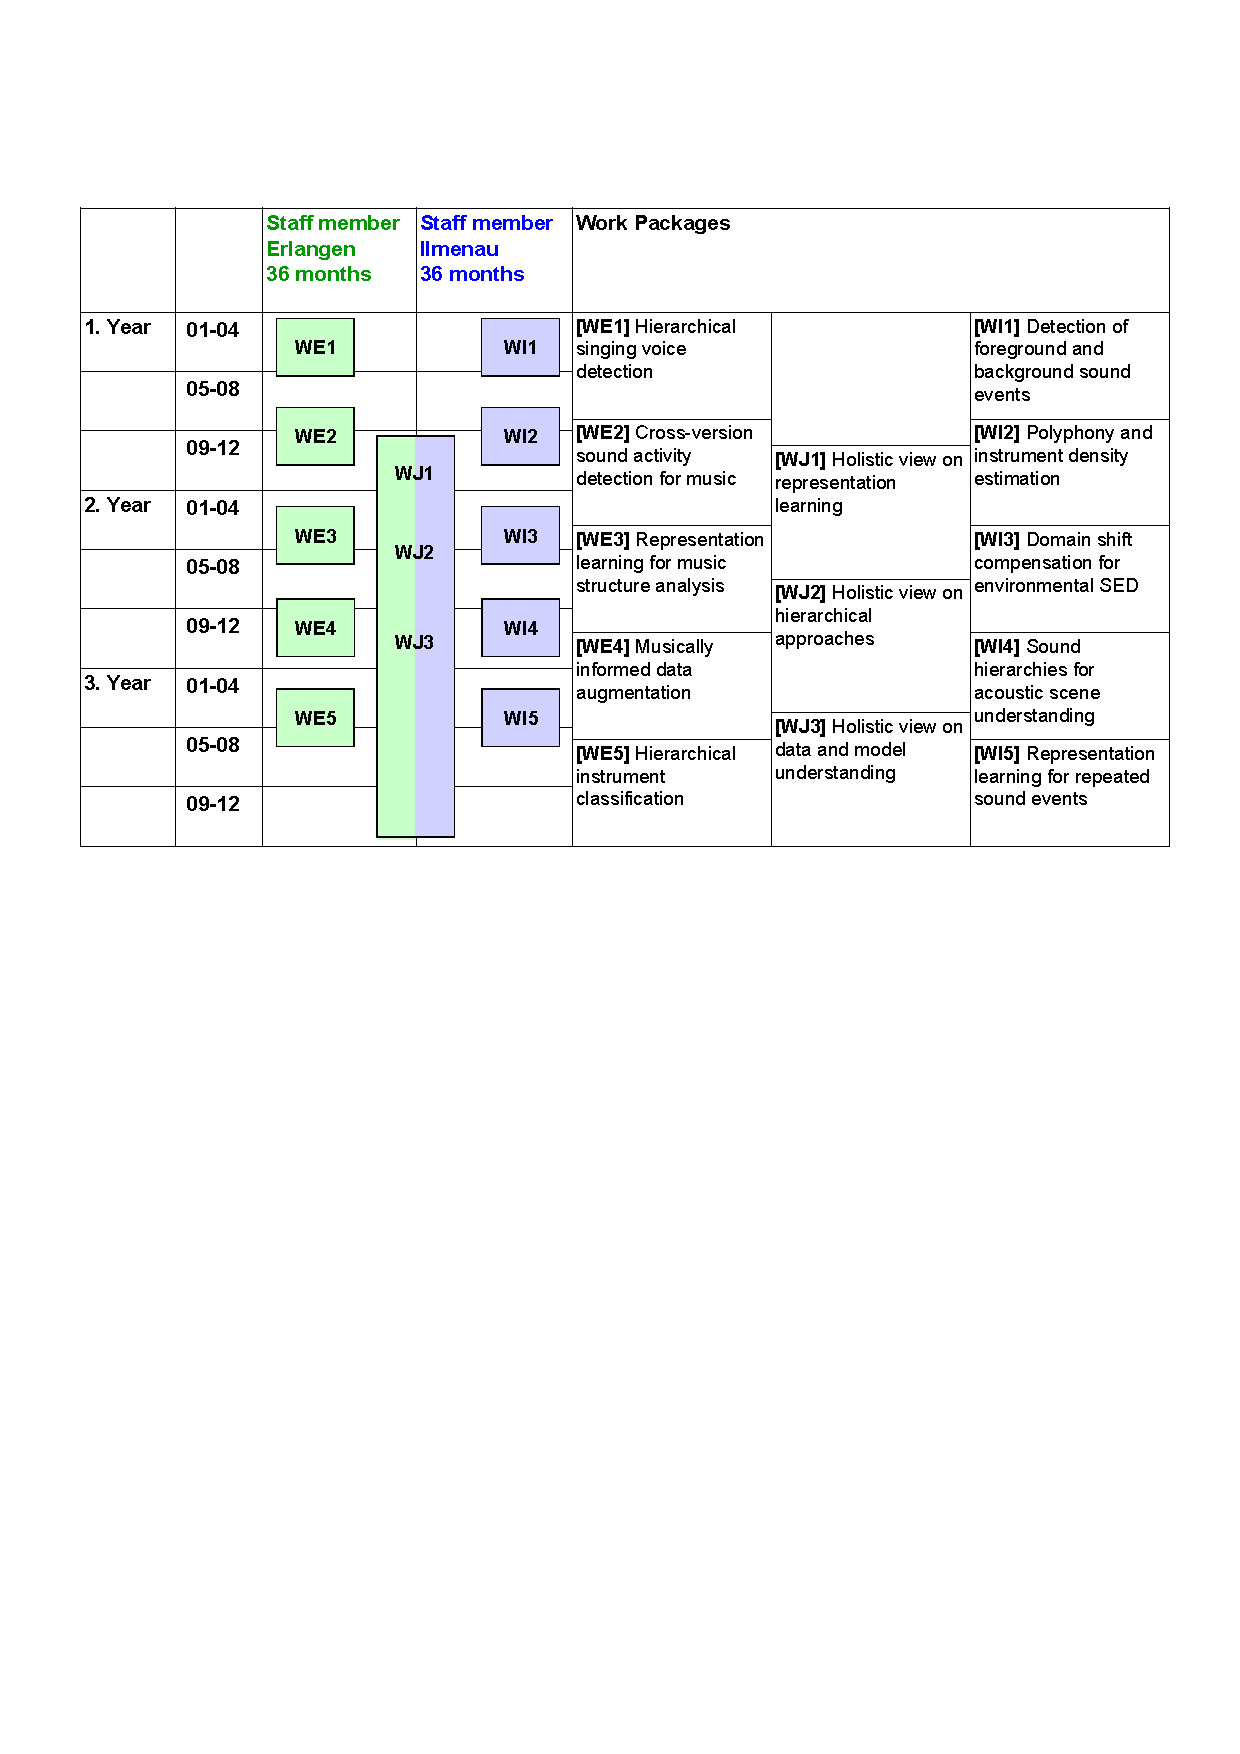
\includegraphics[width=13cm]{2021_MuellerAbesser_DFG-Antrag_ActDet_Timetable.pdf}
\end{center}
\vspace{-0.3cm}
\caption{
Overview of the rough temporal arrangement of the work packages of the $\PN$~project's second phase (renewal proposal). 
%It is estimated that the scientific staff member addresses each of the work packages for roughly four to five months in total. Note that the work packages may be dealt with in a parallel, overlapping or interlocked fashion. Throughout the $\PN$~project, the scientific staff member is supported by two student assistants.
}
\label{figures:AP}
\end{figure}

%%%%%%%%%%%%%%%%%%%%%%%%%%%%%%%%%%%%%%%%%%%%%%%%%%%%%%%%%%%%%%%%%%%%%
\section*{3 Bibliography concerning the state of the art, the research objectives, and the work programme}
%\label{section:Literaturverzeichnis}
%%%%%%%%%%%%%%%%%%%%%%%%%%%%%%%%%%%%%%%%%%%%%%%%%%%%%%%%%%%%%%%%%%%%%

%%%%%%%%%%%%%%%%%%%%%%%%%%%%%%%%%%%%%%%%%%%%%%%%%%%%%%%%%%%%%%%%%%%%%%%%%%%%
\renewcommand{\refname}{}
\vspace*{-1cm}
{
\bibliographystyle{siam}
%\itemsep0mm
\footnotesize
%\bibliography{referencesMusic,referencesUnclear}
\bibliography{referencesMusic,referencesNew_MM,referencesNew_JA}
%\printbibliography
}
%%%%%%%%%%%%%%%%%%%%%%%%%%%%%%%%%%%%%%%%%%%%%%%%%%%%%%%%%%%%%%%%%%%%%%%%%%%%

\pagebreak[4]

%%%%%%%%%%%%%%%%%%%%%%%%%%%%%%%%%%%%%%%%%%%%%%%%%%%%%%%%%%%%%%%%%%%%%
\section*{4 Relevance of sex, gender and/or diversity}
%\label{section:Mittel}
%%%%%%%%%%%%%%%%%%%%%%%%%%%%%%%%%%%%%%%%%%%%%%%%%%%%%%%%%%%%%%%%%%%%%

Both research groups in Erlangen (FAU) and Ilmenau (IDMT) actively strive for diversity concerning various dimensions, including gender, cultural background, and research disciplines. Assuming an open, international, and interdisciplinary perspective is a core element of this project, which is also reflected by applicants' international research and teaching activities and cross-disciplinary collaborations (including computer science, electrical engineering, cognitive sciences, musicology, and acoustics).

%%%%%%%%%%%%%%%%%%%%%%%%%%%%%%%%%%%%%%%%%%%%%%%%%%%%%%%%%%%%%%%%%%%%%
\section*{5 Supplementary information on the research context}
%\label{section:Mittel}
%%%%%%%%%%%%%%%%%%%%%%%%%%%%%%%%%%%%%%%%%%%%%%%%%%%%%%%%%%%%%%%%%%%%%

%%%%%%%%%%%%%%%%%%%%%%%%%%%%%%%%%%%%%%%%%%%%%%%%%%%%%%%%%%%%%%%%%%%%%
\subsection*{5.1 Ethical and/or legal aspects of the project}
%\label{section:Mittel}
%%%%%%%%%%%%%%%%%%%%%%%%%%%%%%%%%%%%%%%%%%%%%%%%%%%%%%%%%%%%%%%%%%%%%
%
\vspace{-0.4cm}
Not applicable.
\vspace{-0.4cm}

%%%%%%%%%%%%%%%%%%%%%%%%%%%%%%%%%%%%%%%%%%%%%%%%%%%%%%%%%%%%%%%%%%%%%
\subsection*{5.1.1 Ethical and/or legal aspects of the project}
%\label{section:Mittel}
%%%%%%%%%%%%%%%%%%%%%%%%%%%%%%%%%%%%%%%%%%%%%%%%%%%%%%%%%%%%%%%%%%%%%
%
\vspace{-0.4cm}
Not applicable.
\vspace{-0.4cm}


%%%%%%%%%%%%%%%%%%%%%%%%%%%%%%%%%%%%%%%%%%%%%%%%%%%%%%%%%%%%%%%%%%%%%
\subsection*{5.1.2 Descriptions of proposed investigations involving experiments on humans or human materials}
%\label{section:Mittel}
%%%%%%%%%%%%%%%%%%%%%%%%%%%%%%%%%%%%%%%%%%%%%%%%%%%%%%%%%%%%%%%%%%%%%
%
\vspace{-0.4cm}
Not applicable.
\vspace{-0.4cm}


%%%%%%%%%%%%%%%%%%%%%%%%%%%%%%%%%%%%%%%%%%%%%%%%%%%%%%%%%%%%%%%%%%%%%
\subsection*{5.1.3 Descriptions of proposed investigations involving experiments on animals}
%\label{section:Mittel}
%%%%%%%%%%%%%%%%%%%%%%%%%%%%%%%%%%%%%%%%%%%%%%%%%%%%%%%%%%%%%%%%%%%%%
%
\vspace{-0.4cm}
Not applicable.
\vspace{-0.4cm}

%%%%%%%%%%%%%%%%%%%%%%%%%%%%%%%%%%%%%%%%%%%%%%%%%%%%%%%%%%%%%%%%%%%%%
\subsection*{5.1.4 Descriptions of projects involving genetic resources (or associated traditional knowledge) from a foreign country}
%\label{section:Mittel}
%%%%%%%%%%%%%%%%%%%%%%%%%%%%%%%%%%%%%%%%%%%%%%%%%%%%%%%%%%%%%%%%%%%%%
%
\vspace{-0.4cm}
Not applicable.
\vspace{-0.4cm}


%%%%%%%%%%%%%%%%%%%%%%%%%%%%%%%%%%%%%%%%%%%%%%%%%%%%%%%%%%%%%%%%%%%%%
\subsection*{5.1.5 Descriptions of investigations involving dual use research of concern, foreign trade regulations}
%\label{section:Mittel}
%%%%%%%%%%%%%%%%%%%%%%%%%%%%%%%%%%%%%%%%%%%%%%%%%%%%%%%%%%%%%%%%%%%%%
%
\vspace{-0.4cm}
Not applicable.
\vspace{-0.4cm}


%%%%%%%%%%%%%%%%%%%%%%%%%%%%%%%%%%%%%%%%%%%%%%%%%%%%%%%%%%%%%%%%%%%%%
\subsection*{5.2 Data handling}
%\label{section:Mittel}
%%%%%%%%%%%%%%%%%%%%%%%%%%%%%%%%%%%%%%%%%%%%%%%%%%%%%%%%%%%%%%%%%%%%%
%
\vspace{-0.4cm}
To promote the reproducibility of scientific research, we intend to focus on publicly available resources. In particular, we will use publicly available environmental sound datasets such as those from the \emph{``Detection and Classification of Acoustic Scenes and Events''} (DCASE) campaign\footnote{\url{http://dcase.community/}}.
%
As in the first phase, we make additional annotations, research results, demonstrators, sound examples, and source code publicly available on suitable websites and repositories such as Github\footnote{\url{https://github.com/}}.
\vspace{-0.4cm}
%
%These resources are described in the paragraph on ``Datasets'' of Section~1.
%(State of the Art and Preliminary Work).
%(see (W\ref{WP:ReflectEval})).
%\jakob{To promote the reproducibility of scientific research, we intend to focus on publicly available data resources. This holds true for both the music datasets as well as the environmental sound datasets, many of which have been published as part of the Detection and Classification of Acoustic Scenes and Events (DCASE) campaign\footnote{\url{http://dcase.community/}} in recent years. 
%
%As in the first phase of the $\PN$-project, we will make additional annotations as well as segmentation/detection results publicly available on our project website\footnote{\url{https://dfg-isad.github.io/}}. Similarly, we will continue to publish demonstrators, sound examples, and suitable source code for experiment reproduction on publically avaible repositories such as Github\footnote{\url{https://github.com/}}. }
%
% \meinard{We need to overwork the following paragraph. We may also mention github and zenodo.
% %
% In view of reproducibility issues, we mainly want to use data resources that are publicly available. This particularly holds for the new datasets for the research on environmental sounds. As in the first phase of the $\PN$-project, we will make additional annotations as well as segmentation/detection results publicly available on a suitable project website. Furthermore, we plan to have publicly accessible websites with demonstrators, numerous sound examples, and suitable source code. 
% }

%%%%%%%%%%%%%%%%%%%%%%%%%%%%%%%%%%%%%%%%%%%%%%%%%%%%%%%%%%%%%%%%%%%%%
\subsection*{5.3 Other information}
%\label{section:Mittel}
%%%%%%%%%%%%%%%%%%%%%%%%%%%%%%%%%%%%%%%%%%%%%%%%%%%%%%%%%%%%%%%%%%%%%
%
\vspace{-0.4cm}
Not applicable.
\vspace{-0.4cm}


%%%%%%%%%%%%%%%%%%%%%%%%%%%%%%%%%%%%%%%%%%%%%%%%%%%%%%%%%%%%%%%%%%%%%
\section*{6 People/collaborations/funding}
%\label{section:Mittel}
%%%%%%%%%%%%%%%%%%%%%%%%%%%%%%%%%%%%%%%%%%%%%%%%%%%%%%%%%%%%%%%%%%%%%

%%%%%%%%%%%%%%%%%%%%%%%%%%%%%%%%%%%%%%%%%%%%%%%%%%%%%%%%%%%%%%%%%%%%%
\subsection*{6.1 Employment status information}
%\label{section:Mittel}
%%%%%%%%%%%%%%%%%%%%%%%%%%%%%%%%%%%%%%%%%%%%%%%%%%%%%%%%%%%%%%%%%%%%%
\vspace{-0.4cm}
M\"uller, Meinard, Universit\"atsprofessor (W3), permanent (unbefristet)\\
Abe{\ss}er, Jakob, Senior Scientist (Fraunhofer IDMT, TV\"OD 13) permanent (unbefristet)
\vspace{-0.4cm}

%%%%%%%%%%%%%%%%%%%%%%%%%%%%%%%%%%%%%%%%%%%%%%%%%%%%%%%%%%%%%%%%%%%%%
\subsection*{6.2 First-time proposal data}
%\label{section:Mittel}
%%%%%%%%%%%%%%%%%%%%%%%%%%%%%%%%%%%%%%%%%%%%%%%%%%%%%%%%%%%%%%%%%%%%%
%
\vspace{-0.4cm}
Not applicable.
%\vspace{-0.4cm}


%%%%%%%%%%%%%%%%%%%%%%%%%%%%%%%%%%%%%%%%%%%%%%%%%%%%%%%%%%%%%%%%%%%%%
\subsection*{6.3 Composition of the project group}
%\label{section:Mittel}
%%%%%%%%%%%%%%%%%%%%%%%%%%%%%%%%%%%%%%%%%%%%%%%%%%%%%%%%%%%%%%%%%%%%%

\textbf{Research Group in Erlangen:}
\begin{itemizePacked}
\item Meinard M\"uller, Prof. Dr. rer. nat. (W3, FAU)
\item Christof Wei{\ss}, Dr.-Ing., Postdoc (Wiss. Angestellter, TVL E14, FAU)
%\item Frank Zalkow, Ph.D. student (Wiss. Angestellter, TVL E13, FAU) 
\item Sebastian Rosenzweig, Ph.D. student (Wiss. Angestellter, TVL E13, FAU) 
\item Michael Krause, Ph.D. student (Wiss. Angestellter, TVL E13, FAU)  
\item Yigitcan {\"O}zer, Ph.D. student (Wiss. Angestellter, TVL E13, FAU)  
\end{itemizePacked}

In Erlangen, the following people are expected to contribute to the $\PN$~project:
the project-funded staff member (100\%, 36 months, intended for Michael Krause and a new Ph.D. student),
Prof. Meinard M\"uller (10\%, supervision, organization, project work),
Sebastian Rosenzweig (5\%, project work, synergies to his work on fundamental frequency estimation),
Dr. Christof Wei{\ss} (5\%, project work and supervision, synergies to his work on tonal analysis),
Yigitcan {\"O}zer (5\%, project work, synergies to his work on audio decomposition and synthesis).
%
%Thomas Pr\"atzlich and Jonathan Driedger are expected to graduate in the next months and will leave the group.
%
Furthermore, the infrastructure of the International Audio Laboratories Erlangen can be used
(Dr.~Stefan Turowski, coordinator; Elke Weiland, secretary).
%(Dr.~Stefan Turowski, coordinator; Elke Weiland and Day-See Riechmann, secretary).

\textbf{Research Group in Ilmenau:}
\begin{itemizePacked}
\item Jakob Abe{\ss}er, Dr.-Ing., TV\"OD 13 (Senior Scientist, Fraunhofer IDMT)
\item Hanna Lukashevich, Head of \emph{Semantic Music Technologies} (Fraunhofer IDMT)
\item Michael Taenzer, Ph.D. student (Wiss. Mitarbeiter, Fraunhofer IDMT)
\item Christon Ragavan Nadar, Ph.D. student (Wiss. Mitarbeiter, Fraunhofer IDMT)
\item Sascha Grollmisch, Ph.D. student (Wiss. Mitarbeiter, Fraunhofer IDMT)
\end{itemizePacked}

In Ilmenau (\emph{Semantic Music Technologies} Group at Fraunhofer IDMT), 
the following people are expected to contribute to the $\PN$~project:
the project-funded staff member (100\%, 36 months, intended for Michael Taenzer and Christon Ragavan Nadar),
Dr. Jakob Abe{\ss}er (10\%, supervision, organization, project work),
Hanna Lukashevich (5\%, project work, synergies to her work on machine learning for music information retrieval),
Sascha Grollmisch (5\%, synergies to his work on sound event detection and industrial sound analysis).
%
Furthermore, the infrastructure of the Fraunhofer IDMT Ilmenau can be used.

%%%%%%%%%%%%%%%%%%%%%%%%%%%%%%%%%%%%%%%%%%%%%%%%%%%%%%%%%%%%%%%%%%%%%
\subsection*{6.4 Researchers in Germany with whom you have agreed to cooperate on this project}
%\label{section:Mittel}
%%%%%%%%%%%%%%%%%%%%%%%%%%%%%%%%%%%%%%%%%%%%%%%%%%%%%%%%%%%%%%%%%%%%%


% Prof. Gerald Schuller (TU Ilmenau)\\
% Senior Prof. Karlheinz Brandenburg (TU Ilmenau)\\
Prof. Rainer Kleinertz (Institut f\"ur Musikwissenschaft, Universit\"at des Saarlandes)\\
Prof. Martin Pfleiderer (Hochschule f\"ur Musik, Weimar)\\
Prof. Sebastian Stober (IKS-AiLab, Otto-von-Guericke-Universit{\"a}t Magdeburg)

%%%%%%%%%%%%%%%%%%%%%%%%%%%%%%%%%%%%%%%%%%%%%%%%%%%%%%%%%%%%%%%%%%%%%
\subsection*{6.5 Researchers abroad with whom you have agreed to cooperate on this project}
%\label{section:Mittel}
%%%%%%%%%%%%%%%%%%%%%%%%%%%%%%%%%%%%%%%%%%%%%%%%%%%%%%%%%%%%%%%%%%%%%

Dr. Emmanouil Benetos (Machine Listening Lab, Queen Mary University, London, UK)\\
Prof. Tuomas Virtanen (Audio Research Group, Uni Tampere, Finland)\\
%Dr. Konstantinos Drossos (Audio Research Group, Uni Tampere, Finland)\\
%Prof. Ga{\"e}l Richard (Télécom ParisTech, Paris, France)\\
%Prof. Mark Plumbley (Surrey, UK)\\
Prof. Geoffroy Peeters (T{\'e}l{\'e}com ParisTech, Paris, France)

%%%%%%%%%%%%%%%%%%%%%%%%%%%%%%%%%%%%%%%%%%%%%%%%%%%%%%%%%%%%%%%%%%%%%
\subsection*{6.6 Researchers with whom you have collaborated scientifically within the past three years}
%\label{section:Mittel}
%%%%%%%%%%%%%%%%%%%%%%%%%%%%%%%%%%%%%%%%%%%%%%%%%%%%%%%%%%%%%%%%%%%%%


%Prof. Dr. Meinard Müller (Audiolabs Erlangen)
%Dr. Christof Weiß (Audiolabs Erlangen)
Dr. Stefan Balke (pmOne Group)\\
Prof. Juan P. Bello (New York University)\\
Dr. Estefanía Cano (AudioSourceRe)\\
Prof. Dr. Simon Dixon (Queen Mary University of London, UK)\\
Dr. Klaus Frieler (Max-Planck-Institut für empirische Ästhetik)\\
Prof. Rainer Kleinertz (Universit{\"a}t des Saarlandes)\\
Prof. Alexander Lerch (Georgia Institute of Technology, US)\\
Prof. Martin Pfleiderer (HfM Weimar)\\
Prof. Frank Scherbaum (Universit\"at Potsdam)\\
Prof. Vesa V{\"a}lim{\"a}ki (Aalto University, Finland)\\
%Prof. Dr. Christian Beste (TU Dresden)
%Prof. Dr. Carsten Beta (University of Potsdam)
%David A. Bridwell (Mind Research Network, Albuquerque, USA)
%Vince D. Calhoun, Ph.D. (Center for Translational Research in Neuroimaging and Data Science, USA)
%James F. Cavanagh, Ph.D. (University of New Mexico, Albuquerque, USA)
%Anne G. E. Collins, Ph.D. (UC Berkeley, USA)
%Prof. Dr. Emrah Düzel (German Center for Neurodegenerative Diseases (DZNE), Magdeburg)
%Prof. Dr. Marc Dewey (Charité, Berlin)
%Michael D. Nunez, Ph.D. (UC Irvine, USU)
%Prof. Dr. Andreas Nürnberger (Otto von Guericke University Magdeburg)
%Jun.-Prof. Dr. Kerstin Ritter (Charité, Berlin)
%Prof. Dr. Harald Sack (FIZ Karlsruhe)
%Ramesh Srinivasan, Ph.D. (UC Irvine, USA)
%Prof. Dr. Manfred Stede (University of Potsdam)
%Prof. Dr. Henrik Walter (Charité, Berlin)
Prof. Sebastian Stober (Otto-von-Guericke-Universit{\"a}t Magdeburg)\\
Prof. Gerhard Widmer (Johannes Kepler University Linz, Austria)

%%%%%%%%%%%%%%%%%%%%%%%%%%%%%%%%%%%%%%%%%%%%%%%%%%%%%%%%%%%%%%%%%%%%%
\subsection*{6.7 Project-relevant cooperation with commercial enterprises}
%\label{section:Mittel}
%%%%%%%%%%%%%%%%%%%%%%%%%%%%%%%%%%%%%%%%%%%%%%%%%%%%%%%%%%%%%%%%%%%%%
%
\vspace{-0.4cm}
Not applicable.
\vspace{-0.4cm}


%%%%%%%%%%%%%%%%%%%%%%%%%%%%%%%%%%%%%%%%%%%%%%%%%%%%%%%%%%%%%%%%%%%%%
\subsection*{6.8 Project-relevant participation in commercial enterprises}
%\label{section:Mittel}
%%%%%%%%%%%%%%%%%%%%%%%%%%%%%%%%%%%%%%%%%%%%%%%%%%%%%%%%%%%%%%%%%%%%%
%
\vspace{-0.4cm}
Not applicable.
\vspace{-0.4cm}


%%%%%%%%%%%%%%%%%%%%%%%%%%%%%%%%%%%%%%%%%%%%%%%%%%%%%%%%%%%%%%%%%%%%%
\subsection*{6.9 Scientific equipment}
%\label{section:Mittel}
%%%%%%%%%%%%%%%%%%%%%%%%%%%%%%%%%%%%%%%%%%%%%%%%%%%%%%%%%%%%%%%%%%%%%
%
\vspace{-0.4cm}
All scientific equipment required for this project (hardware, software) is available
\vspace{-0.4cm}



%%%%%%%%%%%%%%%%%%%%%%%%%%%%%%%%%%%%%%%%%%%%%%%%%%%%%%%%%%%%%%%%%%%%%
\subsection*{6.10 Other submissions}
%\label{section:Mittel}
%%%%%%%%%%%%%%%%%%%%%%%%%%%%%%%%%%%%%%%%%%%%%%%%%%%%%%%%%%%%%%%%%%%%%
%
\vspace{-0.4cm}
No other application for funding of this project has been submitted.
If we make such a proposal, we will immediately inform the German Research Foundation.
\vspace{-0.4cm}




%%%%%%%%%%%%%%%%%%%%%%%%%%%%%%%%%%%%%%%%%%%%%%%%%%%%%%%%%%%%%%%%%%%%%
\section*{7 Requested modules/funds}
%%%%%%%%%%%%%%%%%%%%%%%%%%%%%%%%%%%%%%%%%%%%%%%%%%%%%%%%%%%%%%%%%%%%%

%%%%%%%%%%%%%%%%%%%%%%%%%%%%%%%%%%%%%%%%%%%%%%%%%%%%%%%%%%%%%%%%%%%%%
\subsection*{7.1 Basic module}
%%%%%%%%%%%%%%%%%%%%%%%%%%%%%%%%%%%%%%%%%%%%%%%%%%%%%%%%%%%%%%%%%%%%%

%%%%%%%%%%%%%%%%%%%%%%%%%%%%%%%%%%%%%%%%%%%%%%%%%%%%%%%%%%%%%%%%%%%%%
\subsubsection*{7.1.1 Funding for staff}
%%%%%%%%%%%%%%%%%%%%%%%%%%%%%%%%%%%%%%%%%%%%%%%%%%%%%%%%%%%%%%%%%%%%%

\paragraph*{Scientific staff (full position, TVL 13, 36 months, Erlangen).}
The staff member takes over the work for Erlangen throughout the total duration of the project. She/he needs to have excellent qualifications in the areas of Music Information Retrieval, Digital Signal Processing, and Machine Learning. Furthermore, comprehensive programming skills in Python are required. Basic musicological knowledge is requested.
%
A highly qualified candidate for this position is Michael Krause, who already worked in the first phase of the $\PN$-project. The DFG position would allow him to concentrate on his research while finishing his Ph.D. (third and fourth year). Furthermore, we plan to hire a new Ph.D. student joining the $\PN$-project at the beginning of her/his Ph.D.

\paragraph*{Scientific staff (full position, TV{\"O}D 13, 36 months, Ilmenau).}
The staff member takes over the work in Ilmenau throughout the total duration of the project. She/he needs to have excellent qualifications in the areas of Audio Signal Processing and Machine Learning with a focus on Deep Learning. Furthermore, very good programming skills in Python including prior knowledge of common machine learning libraries such as scikit-learn, keras, tensorflow, or pytorch are required.
%
Two highly qualified candidates to share this position are Michael Taenzer (already funded by the $\PN$-project in its first phase) and Christon Ragavan Nadar (a former master student jointly supervised by Ilmenau and Erlangen). The DFG position would allow Mr. Taenzer to finishing his Ph.D. (fourth and fifth year) and Mr. Nadar to start his Ph.D. joining the $\PN$-project.
%
%The DFG position would allow Mr. Taenzer to conduct further research related to instrument recognition and polyphony estimation while finishing his Ph.D. (fourth and fifth year) and Mr. Nadar to activly contribute to both MIR and ESA research topics.

\paragraph*{Four student assistants (\`a 36 months \`a 40h/month, Erlangen and Ilmenau).}
To support the staff members, we ask for four student assistants (two for Erlangen and two for Ilmenau) with excellent
programming skills (in particular Python and/or Java) and a good musical background. 
%
The student assistants are required for several research-related tasks.
First, prototypical interfaces and web-based demonstrators for the applications are to be developed and implemented.
Second, standard signal processing and machine learning algorithms from the scientific literature
need to be (re-)implemented, adapted, and tested.
Third, datasets and annotations need to be maintained and generated.
Fourth, evaluations and tests are to be conducted.
%
One superordinate goal of the $\PN$~project is to introduce motivated students to current research problems at an early stage of their studies. This can be achieved by integrating them into the research group by means of student assistant positions, which may then lead to Master and Bachelor thesis projects related to the $\PN$~project.


%%%%%%%%%%%%%%%%%%%%%%%%%%%%%%%%%%%%%%%%%%%%%%%%%%%%%%%%%%%%%%%%%%%%%
\subsubsection*{7.1.2 Direct Project Costs}
%%%%%%%%%%%%%%%%%%%%%%%%%%%%%%%%%%%%%%%%%%%%%%%%%%%%%%%%%%%%%%%%%%%%%

%%%%%%%%%%%%%%%%%%%%%%%%%%%%%%%%%%%%%%%%%%%%%%%%%%%%%%%%%%%%%%%%%%%%%
\paragraph*{7.1.2.1	Equipment up to EUR 10,000, Software and Consumables.}
%%%%%%%%%%%%%%%%%%%%%%%%%%%%%%%%%%%%%%%%%%%%%%%%%%%%%%%%%%%%%%%%%%%%%
%
Not applicable.
\vspace{-0.4cm}


%%%%%%%%%%%%%%%%%%%%%%%%%%%%%%%%%%%%%%%%%%%%%%%%%%%%%%%%%%%%%%%%%%%%%
\paragraph*{7.1.2.2	Travel Expenses.}
%%%%%%%%%%%%%%%%%%%%%%%%%%%%%%%%%%%%%%%%%%%%%%%%%%%%%%%%%%%%%%%%%%%%%
%
The expected research results should be published and presented at major international conferences (\egc ICASSP, ISMIR, EUSIPCO, ACM Multimedia, WASPAA, AES). Per year, we expect that each of the two staff members visits two major conferences (with an estimated cost of EUR 2000 per conference comprising overseas flight, hotel, and registration fee) and several smaller conferences, workshops, and visits of the project partners. This amounts to an estimated cost of EUR 5000 per year and per staff member. Over three years, this results in the following estimation for travel expenses:
\hfill{\underline{EUR 30000}}\\
%
\vspace{-0.4cm}

%%%%%%%%%%%%%%%%%%%%%%%%%%%%%%%%%%%%%%%%%%%%%%%%%%%%%%%%%%%%%%%%%%%%%
\paragraph*{7.1.2.3	Visiting Researchers (excluding Mercator Fellows).} 
%%%%%%%%%%%%%%%%%%%%%%%%%%%%%%%%%%%%%%%%%%%%%%%%%%%%%%%%%%%%%%%%%%%%%
%
We would like to invite at least one guest scientist per year per project partner for a guest talk and joint research (estimated at 600 EUR per visit), resulting in a total amount of
\hfill{\underline{EUR 3600}}\\
%
\vspace{-0.4cm}

%\meinard{
%The $\PN$~project deals with research questions that are also relevant
%for researchers and students from other disciplines including
%musicology and digital humanities. During the project, we would like
%to organize workshops, tutorials, and seminars in Erlangen and Ilmenau,
%where we can invite internationally renowned colleagues from various fields. 
%Having an interdisciplinary exchange of ideas with colleagues from
%engineering and the humanities not only gives us important feedback
%and perspectives for the $\PN$~project, but may also foster future, larger-scaled
%collaborative projects. Such activities are also essential for further establishing MIR
%within Germany. 
%}
%To this end, the estimated costs are EUR 2000 (travel expenses and hotel) per year,
%resulting in a total amount of
%\hfill{\underline{EUR 6000}\\

%%%%%%%%%%%%%%%%%%%%%%%%%%%%%%%%%%%%%%%%%%%%%%%%%%%%%%%%%%%%%%%%%%%%%
\paragraph*{7.1.2.4	Expenses for Laboratory Animals.}
%%%%%%%%%%%%%%%%%%%%%%%%%%%%%%%%%%%%%%%%%%%%%%%%%%%%%%%%%%%%%%%%%%%%%
%
Not applicable.
\vspace{-0.4cm}

%%%%%%%%%%%%%%%%%%%%%%%%%%%%%%%%%%%%%%%%%%%%%%%%%%%%%%%%%%%%%%%%%%%%%
\paragraph*{7.1.2.5	Other Costs.}
%%%%%%%%%%%%%%%%%%%%%%%%%%%%%%%%%%%%%%%%%%%%%%%%%%%%%%%%%%%%%%%%%%%%%
%
Not applicable.
\vspace{-0.4cm}}

%%%%%%%%%%%%%%%%%%%%%%%%%%%%%%%%%%%%%%%%%%%%%%%%%%%%%%%%%%%%%%%%%%%%%
\paragraph*{7.1.2.6	Project-Related Publication Expenses.} 
%%%%%%%%%%%%%%%%%%%%%%%%%%%%%%%%%%%%%%%%%%%%%%%%%%%%%%%%%%%%%%%%%%%%%
%
Open-access articles in renowned peer-reviewed journals are subject to a fee (between 500 and 1500 EUR per article). To this end, we request the following allowance:\hfill{\underline{EUR 6000}}
\vspace{-0.4cm}

%%%%%%%%%%%%%%%%%%%%%%%%%%%%%%%%%%%%%%%%%%%%%%%%%%%%%%%%%%%%%%%%%%%%%
\subsubsection*{7.1.3 Instrumentation}
%%%%%%%%%%%%%%%%%%%%%%%%%%%%%%%%%%%%%%%%%%%%%%%%%%%%%%%%%%%%%%%%%%%%%
%
\vspace{-0.4cm}
Not applicable.
\vspace{-0.4cm}

%%%%%%%%%%%%%%%%%%%%%%%%%%%%%%%%%%%%%%%%%%%%%%%%%%%%%%%%%%%%%%%%%%%%%
\subsection*{7.2 Module workshop funding}
%%%%%%%%%%%%%%%%%%%%%%%%%%%%%%%%%%%%%%%%%%%%%%%%%%%%%%%%%%%%%%%%%%%%%
%
\vspace{-0.4cm}
As a platform to present and discuss project results, we plan to host an international research workshop in 
Ilmenau/Erfurt or Erlangen in the year 2023. In addition to the $\PN$-project's doctoral students and PIs, also Master and Bachelor students will get the opportunity to present their results. Furthermore, we plan to have several invited speakers and experts from other leading (international) institutes. While discussing scientific results and obtaining feedback from outside, the main goal of this workshop to develop further research questions and stimulate collaborations with other research institutions. For organizing this workshop, we request the following allowance: 1.) Travel expenses for four international guest speakers (EUR 500 per person). 2.) Travel expenses for four domestic guest speakers (EUR 150 per person). 3.) Two overnight stays for all eight speakers (EUR 100 per night per guest). This results in a total amount of \hfill{\underline{EUR 4200}}

%\begin{table}[h!]
%\centering
%\begin{tabular}{lrrr}
% Travel costs foreign countries & 4 $\times$ & 500 EUR & 2,000 EUR  \\
%  Domestic travel expenses & 4 $\times$ & 100 EUR & 400 EUR  \\
% Two overnight stays & 8 $\times$ & 150 EUR & 1,200 EUR  \\
% \hline
% \textbf{Total} &  &  &  \textbf{3,600 EUR}  \\
%\end{tabular}
%\end{table}

%%%%%%%%%%%%%%%%%%%%%%%%%%%%%%%%%%%%%%%%%%%%%%%%%%%%%%%%%%%%%%%%%%%%%
\subsection*{7.3 Module public relations funding}
%%%%%%%%%%%%%%%%%%%%%%%%%%%%%%%%%%%%%%%%%%%%%%%%%%%%%%%%%%%%%%%%%%%%%
%
\vspace{-0.4cm}
Not applicable.
\vspace{-0.4cm}

\end{document}
